\documentclass[]{article}
\usepackage{lmodern}
\usepackage{amssymb,amsmath}
\usepackage{ifxetex,ifluatex}
\usepackage{fixltx2e} % provides \textsubscript
\ifnum 0\ifxetex 1\fi\ifluatex 1\fi=0 % if pdftex
  \usepackage[T1]{fontenc}
  \usepackage[utf8]{inputenc}
\else % if luatex or xelatex
  \ifxetex
    \usepackage{mathspec}
  \else
    \usepackage{fontspec}
  \fi
  \defaultfontfeatures{Ligatures=TeX,Scale=MatchLowercase}
\fi
% use upquote if available, for straight quotes in verbatim environments
\IfFileExists{upquote.sty}{\usepackage{upquote}}{}
% use microtype if available
\IfFileExists{microtype.sty}{%
\usepackage{microtype}
\UseMicrotypeSet[protrusion]{basicmath} % disable protrusion for tt fonts
}{}
\usepackage[margin=1in]{geometry}
\usepackage{hyperref}
\hypersetup{unicode=true,
            pdftitle={TUN Data Challenge 2018 : Bike MS},
            pdfauthor={Jordan Beary, Ramya Priya Guntipalli, Konrad Miziolek, Eva Forrester},
            pdfborder={0 0 0},
            breaklinks=true}
\urlstyle{same}  % don't use monospace font for urls
\usepackage{color}
\usepackage{fancyvrb}
\newcommand{\VerbBar}{|}
\newcommand{\VERB}{\Verb[commandchars=\\\{\}]}
\DefineVerbatimEnvironment{Highlighting}{Verbatim}{commandchars=\\\{\}}
% Add ',fontsize=\small' for more characters per line
\usepackage{framed}
\definecolor{shadecolor}{RGB}{248,248,248}
\newenvironment{Shaded}{\begin{snugshade}}{\end{snugshade}}
\newcommand{\KeywordTok}[1]{\textcolor[rgb]{0.13,0.29,0.53}{\textbf{#1}}}
\newcommand{\DataTypeTok}[1]{\textcolor[rgb]{0.13,0.29,0.53}{#1}}
\newcommand{\DecValTok}[1]{\textcolor[rgb]{0.00,0.00,0.81}{#1}}
\newcommand{\BaseNTok}[1]{\textcolor[rgb]{0.00,0.00,0.81}{#1}}
\newcommand{\FloatTok}[1]{\textcolor[rgb]{0.00,0.00,0.81}{#1}}
\newcommand{\ConstantTok}[1]{\textcolor[rgb]{0.00,0.00,0.00}{#1}}
\newcommand{\CharTok}[1]{\textcolor[rgb]{0.31,0.60,0.02}{#1}}
\newcommand{\SpecialCharTok}[1]{\textcolor[rgb]{0.00,0.00,0.00}{#1}}
\newcommand{\StringTok}[1]{\textcolor[rgb]{0.31,0.60,0.02}{#1}}
\newcommand{\VerbatimStringTok}[1]{\textcolor[rgb]{0.31,0.60,0.02}{#1}}
\newcommand{\SpecialStringTok}[1]{\textcolor[rgb]{0.31,0.60,0.02}{#1}}
\newcommand{\ImportTok}[1]{#1}
\newcommand{\CommentTok}[1]{\textcolor[rgb]{0.56,0.35,0.01}{\textit{#1}}}
\newcommand{\DocumentationTok}[1]{\textcolor[rgb]{0.56,0.35,0.01}{\textbf{\textit{#1}}}}
\newcommand{\AnnotationTok}[1]{\textcolor[rgb]{0.56,0.35,0.01}{\textbf{\textit{#1}}}}
\newcommand{\CommentVarTok}[1]{\textcolor[rgb]{0.56,0.35,0.01}{\textbf{\textit{#1}}}}
\newcommand{\OtherTok}[1]{\textcolor[rgb]{0.56,0.35,0.01}{#1}}
\newcommand{\FunctionTok}[1]{\textcolor[rgb]{0.00,0.00,0.00}{#1}}
\newcommand{\VariableTok}[1]{\textcolor[rgb]{0.00,0.00,0.00}{#1}}
\newcommand{\ControlFlowTok}[1]{\textcolor[rgb]{0.13,0.29,0.53}{\textbf{#1}}}
\newcommand{\OperatorTok}[1]{\textcolor[rgb]{0.81,0.36,0.00}{\textbf{#1}}}
\newcommand{\BuiltInTok}[1]{#1}
\newcommand{\ExtensionTok}[1]{#1}
\newcommand{\PreprocessorTok}[1]{\textcolor[rgb]{0.56,0.35,0.01}{\textit{#1}}}
\newcommand{\AttributeTok}[1]{\textcolor[rgb]{0.77,0.63,0.00}{#1}}
\newcommand{\RegionMarkerTok}[1]{#1}
\newcommand{\InformationTok}[1]{\textcolor[rgb]{0.56,0.35,0.01}{\textbf{\textit{#1}}}}
\newcommand{\WarningTok}[1]{\textcolor[rgb]{0.56,0.35,0.01}{\textbf{\textit{#1}}}}
\newcommand{\AlertTok}[1]{\textcolor[rgb]{0.94,0.16,0.16}{#1}}
\newcommand{\ErrorTok}[1]{\textcolor[rgb]{0.64,0.00,0.00}{\textbf{#1}}}
\newcommand{\NormalTok}[1]{#1}
\usepackage{longtable,booktabs}
\usepackage{graphicx,grffile}
\makeatletter
\def\maxwidth{\ifdim\Gin@nat@width>\linewidth\linewidth\else\Gin@nat@width\fi}
\def\maxheight{\ifdim\Gin@nat@height>\textheight\textheight\else\Gin@nat@height\fi}
\makeatother
% Scale images if necessary, so that they will not overflow the page
% margins by default, and it is still possible to overwrite the defaults
% using explicit options in \includegraphics[width, height, ...]{}
\setkeys{Gin}{width=\maxwidth,height=\maxheight,keepaspectratio}
\IfFileExists{parskip.sty}{%
\usepackage{parskip}
}{% else
\setlength{\parindent}{0pt}
\setlength{\parskip}{6pt plus 2pt minus 1pt}
}
\setlength{\emergencystretch}{3em}  % prevent overfull lines
\providecommand{\tightlist}{%
  \setlength{\itemsep}{0pt}\setlength{\parskip}{0pt}}
\setcounter{secnumdepth}{0}
% Redefines (sub)paragraphs to behave more like sections
\ifx\paragraph\undefined\else
\let\oldparagraph\paragraph
\renewcommand{\paragraph}[1]{\oldparagraph{#1}\mbox{}}
\fi
\ifx\subparagraph\undefined\else
\let\oldsubparagraph\subparagraph
\renewcommand{\subparagraph}[1]{\oldsubparagraph{#1}\mbox{}}
\fi

%%% Use protect on footnotes to avoid problems with footnotes in titles
\let\rmarkdownfootnote\footnote%
\def\footnote{\protect\rmarkdownfootnote}

%%% Change title format to be more compact
\usepackage{titling}

% Create subtitle command for use in maketitle
\newcommand{\subtitle}[1]{
  \posttitle{
    \begin{center}\large#1\end{center}
    }
}

\setlength{\droptitle}{-2em}
  \title{TUN Data Challenge 2018 : Bike MS}
  \pretitle{\vspace{\droptitle}\centering\huge}
  \posttitle{\par}
  \author{Jordan Beary, Ramya Priya Guntipalli, Konrad Miziolek, Eva Forrester}
  \preauthor{\centering\large\emph}
  \postauthor{\par}
  \predate{\centering\large\emph}
  \postdate{\par}
  \date{March 23, 2018}


\begin{document}
\maketitle

\hypertarget{github}{%
\subsection{GitHub}\label{github}}

Before getting started please reference the team's GitHub pages for any
and all code related to producing the analysis for this project, which
includes data cleaning scripts, references, data sets, and external
images:

\begin{itemize}
\tightlist
\item
  GitHub Webpage and final report :
  \href{https://github.com/JordanBeary/BikeMS}{JordanBeary}
\item
  Data cleansing and manipulation, data sets, and storing miscellaneous
  files : \href{https://github.com/konradmiz/ETM-527}{konradmiz}
\end{itemize}

\hypertarget{introduction}{%
\section{Introduction}\label{introduction}}

The National Multiple Sclerosis Society (NMSS), founded in 1946, is the
70th largest nonprofit in the United States\footnote{Link to Forbes
  article
  \href{https://www.forbes.com/companies/national-multiple-sclerosis-society/}{Forbes.com}},
and is dedicated to fund research and perform outreach/public awareness
and education regarding Multiple Sclerosis. Multiple Sclerosis (MS), is
more frequent in women than men, and is typically diagnosed in patients
between the ages of 20 and 50\footnote{Read about Multiple Sclerosis at
  \href{https://www.nationalmssociety.org/About-the-Society/MS-Prevalence}{NMSS.org}}.
The causal mechanism of MS is unknown but hypothesized to be an
interplay of an unknown environmental factor and genetic predisposition.
Around 400,000 people in the United States have MS (with an additional
200 diagnosed weekly), and the frequency is about twice as high above
the 37th parallel as below it. As such, Multiple Sclerosis represents a
relevant, impactful disease with a need for research and
education\footnote{Quick MS statistics
  \href{https://www.healthline.com/health/multiple-sclerosis/facts-statistics-infographic}{Healthline}}.

The National Multiple Sclerosis Society raises funds primarily through
individual donations and through sponsored charity bicycle events (Bike
MS) which typically last one or two days\footnote{Visit TUN Data
  Challenge homepage to look at business questions and competition info
  \href{http://www.teradatauniversitynetwork.com/Community/Student-Competitions/2018/Data-Challenge/Business-Questions/}{TUN
  Data Challenge 2018}}. These events occur in the spring, summer, and
fall, and about 70,000 participants take part in one of about 75
different events across the country. As the largest charity bike
fundraiser in the United States, the events collectively raise about
\texttt{\$}68 million. Teams are the largest contributor to the donation
pot, representing about 87\% of the money raised. However, as charities
representing many distinct pathologies now rely on individual donors and
bike rides, the market share for Bike MS has fallen yearly since 2012
and is reflected in declining revenue and numbers of participants.
Retention of past participants is strong, but fewer and fewer new
participants are joining. In 2017, the NMSS suffered a loss of \$8
million\footnote{Link to Forbes article
  \href{https://www.forbes.com/companies/national-multiple-sclerosis-society/}{Forbes.com}}.
To maintain a fundraising advantage and remain competitive in
fundraising, the NMSS has partnered with Teradata University Network to
provide their data and relevant business questions to be addressed.

Multiple Sclerosis defined by the National Multiple Sclerosis
Society\footnote{Read about Multiple Sclerosis at
  \href{https://www.nationalmssociety.org/About-the-Society/MS-Prevalence}{NMSS.org}}:

\begin{quote}
``\ldots{}involves an immune-mediated process in which an abnormal
response of the body's immune system is directed against the central
nervous system (CNS), which is made up of the brain, spinal cord and
optic nerves. The exact antigen --- or target that the immune cells are
sensitized to attack --- remains unknown, which is why MS is considered
by many experts to be `immune-mediated' rather than `autoimmune'\,''

\hfill --- National Multiple Sclerosis Society
\end{quote}

Data on the prevalence of MS is extremely difficult to find, mainly
because it is not consistently reported or required to be reported in
the United States. However, the NMSS trust 2008-2012 estimated
prevalence at around 400,000.

\begin{figure}
\centering
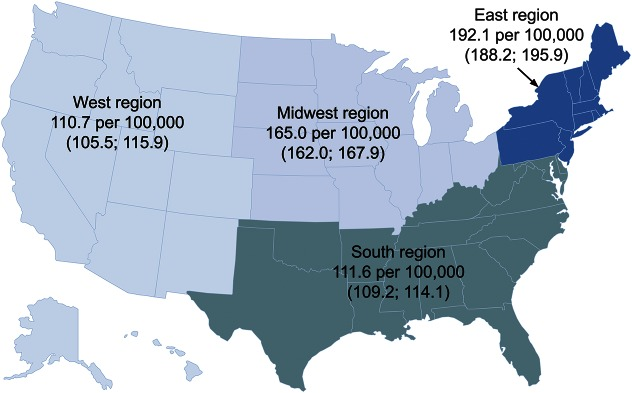
\includegraphics{RegionalMSprev.jpg}
\caption{Regional MS Prevalence}
\end{figure}

Furthermore, a new study is expected to be released this year which
estimates MS incidence and prevalence to be around 1 million in the
United States\footnote{Link to the press release from
  NMSS(\url{https://www.nationalmssociety.org/About-the-Society/News/Preliminary-Results-of-MS-Prevalence-Study})}.
Understanding MS prevalence and those affected by it is critical to
answering why someone would want to join one of the largest cycling
fundraiser in the United States, Bike MS.

\begin{figure}
\centering
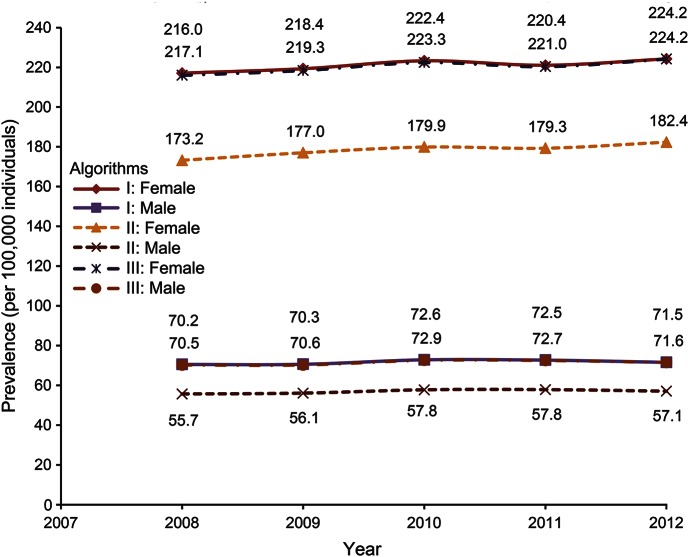
\includegraphics{MSgenderGap.jpg}
\caption{MS Gender Gap}
\end{figure}

Insurance data was collected from 2008 to 2012 and analyzed by the
American Academy of Neurology. The standard prevalence metric is number
of MS patients out of 100,000. There are some interesting trends looking
at gender and geospatial demographics, which could lead to engaging a
population that might be willing to help increase the number of
participants/cyclists and donors. First, approximately 224 out of
100,000 women report living with MS -- compared to just 72 out of
100,000 men. Second, the Eastern Region of the United States has the
highest reported population of insured individuals with MS with 192 out
of 100,000 -- as opposed to 111 our of 100,000 in the Western Region.
With this information, we as analysts can begin generating potential
solutions for the decreasing number of participants and fundraising
efforts for Bike MS.

\hypertarget{business-problem}{%
\section{Business Problem}\label{business-problem}}

The NMSS is primarily interested in increasing the number of corporate
donors: since demographics skew towards middle-aged, white, high-income
earners, Bike MS receives much of its support from large corporate teams
(featuring 10 or more riders). Thus, the overarching business question
to address is how to increase the number of new corporate teams, by
identifying companies with a large employee base and that are aligned
with health/wellness goals. The second is to determine which events and
markets are popular with the corporate demographic and use the knowledge
to better drive event planning.

An additional area of interest is determining the opportunities in
digital marketing for attracting participants and tactically increasing
donations by email reminders, social media advertising, and other
channels. However, this is a secondary goal by the National Multiple
Sclerosis Society.

\hypertarget{business-questions}{%
\section{Business Questions}\label{business-questions}}

\hypertarget{what-are-the-greatest-growth-opportunities-for-new-corporate-teams}{%
\subsection{What are the greatest growth opportunities for new corporate
teams?}\label{what-are-the-greatest-growth-opportunities-for-new-corporate-teams}}

Bike MS has reported that corporate teams with 10+ members are their key
to a successful season of fundraising. They also have a goal of
increasing active registration by almost 9\% from 2017. Last year there
were 74,000 riders and a total of 6,150 teams and their goal for 2018 is
80,572 riders (40,000 new who have not participated within the last five
years), and 6,489 teams. On the Bike MS Business Questions
page\footnote{Visit TUN Data Challenge homepage to look at business
  questions and competition info
  \href{http://www.teradatauniversitynetwork.com/Community/Student-Competitions/2018/Data-Challenge/Business-Questions/}{TUN
  Data Challenge 2018}}, justification for targeting corporate teams:

\begin{quote}
``Because of participant demographics (mostly male, middle age, higher
income earners), we know that Bike MS is an ideal corporate event and
that corporate teams of 10 or more cyclists are seven times more
valuable than any other kind of team. Companies with a large
professional employee base, especially those with a corporate culture of
health and wellness -- regardless of industry -- are key prospects''

\hfill --- Bike MS \& Teradata University Network
\end{quote}

Now we have looked at donations from Fortune 1000 and 500 companies and
estimate that their contribution is not as significant as they might
think. While the summation of donations is large for these companies,
but participants employed by these companies are not more likely to
donate any more than a participant in the Friends and Family division.

\begin{figure}
\centering
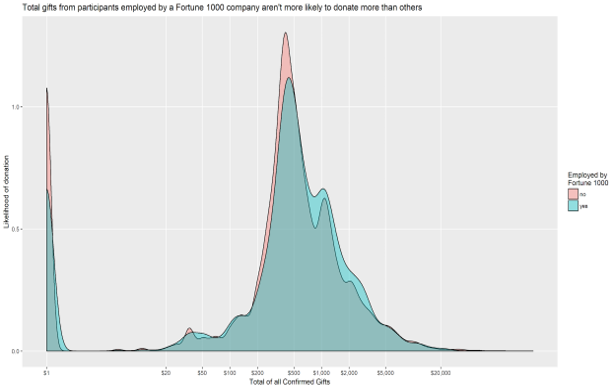
\includegraphics{fortune1000.png}
\caption{Fortune 1000}
\end{figure}

\begin{figure}
\centering
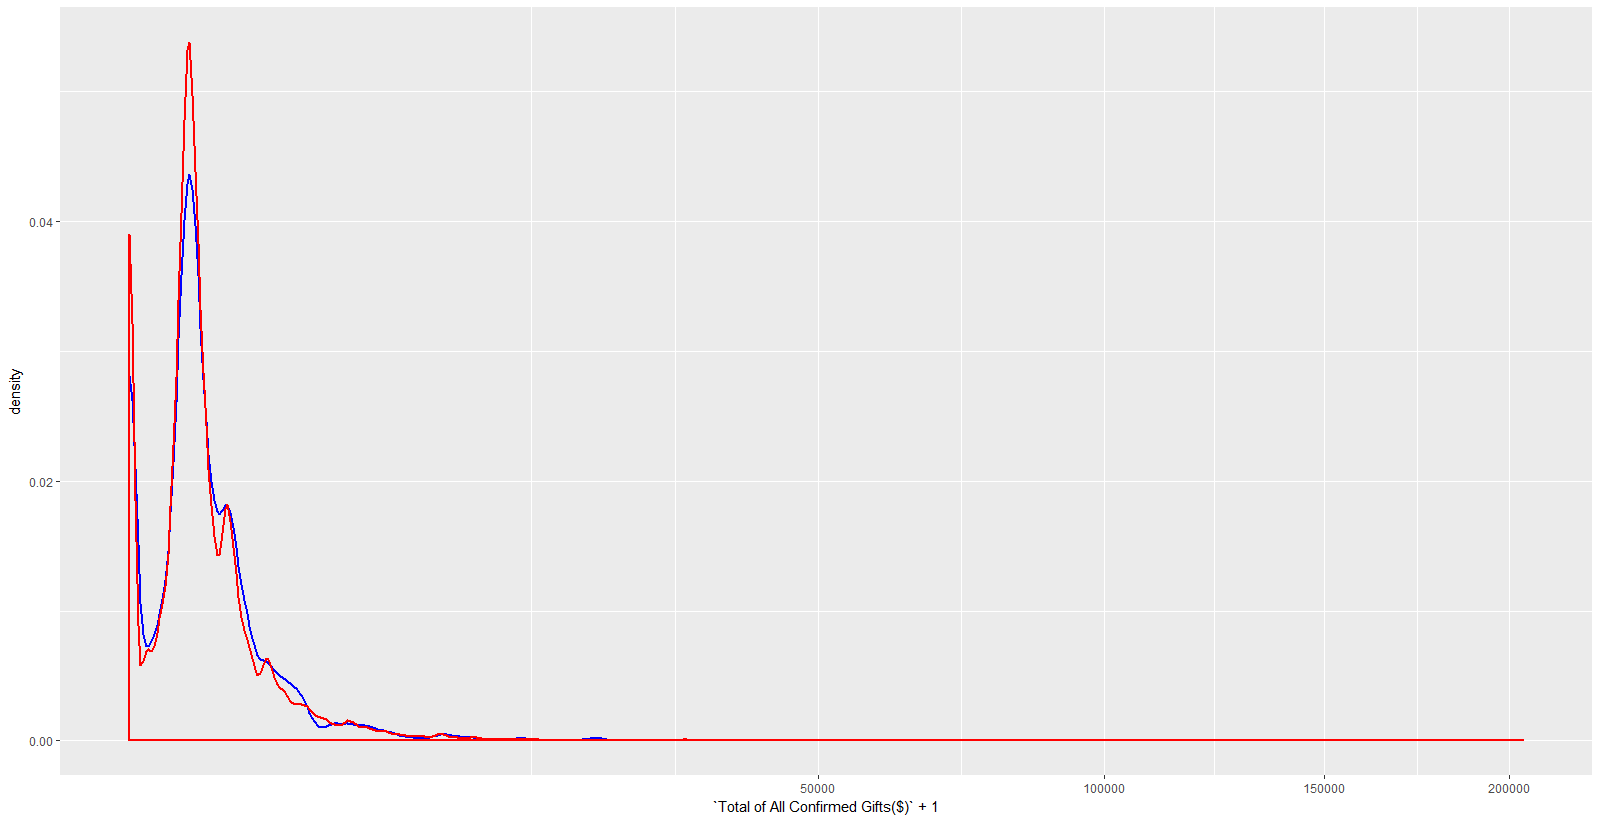
\includegraphics{fortune500.png}
\caption{Fortune 500}
\end{figure}

There is no doubt that corporate teams have a large role to play in the
success of Bike MS, by bringing characteristics like corporate donation
matching, inter-company competition, large teams, and the localization
of generally wealthy individuals. However, In 2017 there were a total of
28.8 million registered small businesses in the United States, with
anywhere from 1 to 5,000 employees. To find specific corporations that
fit the bill of the most successful existing Bike MS corporations might
be a perfectly good way of going about answering this question, but in
my opinion extremely onerous and potentially yield the same fleeting
results each event is experiencing now. Here is where the introductory
information can be used to our advantage. Instead, maybe we should be
thinking from the perspective of a potential donor. What would make
yourself a donor of one fundraiser over another? There is a huge number
of illnesses that impact larger populations of the United States than
the estimated 1 million individuals living with MS. My best guess is
that donors, riders, and volunteers are propelled to Bike MS because of
the personal impact it has had on their own life. These are data-driven
insights - not just assumptions:

\begin{Shaded}
\begin{Highlighting}[]
\NormalTok{participants}\OperatorTok{$}\StringTok{`}\DataTypeTok{Participant Connection to MS}\StringTok{`}\NormalTok{[}\KeywordTok{grep}\NormalTok{(}\StringTok{"MS"}\NormalTok{, participants}\OperatorTok{$}\StringTok{`}\DataTypeTok{Participant Connection to MS}\StringTok{`}\NormalTok{)] <-}\StringTok{ "Direct Connection to MS"}
\NormalTok{participants}\OperatorTok{$}\StringTok{`}\DataTypeTok{Participant Connection to MS}\StringTok{`}\NormalTok{[}\KeywordTok{grep}\NormalTok{(}\StringTok{"Other|other|Relative: Other"}\NormalTok{, }
\NormalTok{    participants}\OperatorTok{$}\StringTok{`}\DataTypeTok{Participant Connection to MS}\StringTok{`}\NormalTok{)] <-}\StringTok{ "Other"}
\NormalTok{participants}\OperatorTok{$}\StringTok{`}\DataTypeTok{Participant Connection to MS}\StringTok{`}\NormalTok{[}\KeywordTok{grep}\NormalTok{(}\StringTok{"Blank|None|No connection|NA"}\NormalTok{, }
\NormalTok{    participants}\OperatorTok{$}\StringTok{`}\DataTypeTok{Participant Connection to MS}\StringTok{`}\NormalTok{)] <-}\StringTok{ "None"}
\NormalTok{participants}\OperatorTok{$}\StringTok{`}\DataTypeTok{Participant Connection to MS}\StringTok{`}\NormalTok{ <-}\StringTok{ }\KeywordTok{as.factor}\NormalTok{(participants}\OperatorTok{$}\StringTok{`}\DataTypeTok{Participant Connection to MS}\StringTok{`}\NormalTok{)}

\NormalTok{bad.states <-}\StringTok{ }\KeywordTok{c}\NormalTok{(}\StringTok{"Dallas"}\NormalTok{, }\StringTok{"Alicante"}\NormalTok{, }\StringTok{"Ardmore"}\NormalTok{, }\StringTok{"Austin"}\NormalTok{, }\StringTok{"Canyon Lake"}\NormalTok{, }
    \StringTok{"Columbia Heights"}\NormalTok{, }\StringTok{"Edinburg"}\NormalTok{, }\StringTok{"Greendale"}\NormalTok{, }\StringTok{"Houston"}\NormalTok{, }\StringTok{"Katy"}\NormalTok{, }
    \StringTok{"Midwest City"}\NormalTok{, }\StringTok{"Minneapolis"}\NormalTok{, }\StringTok{"Morristown"}\NormalTok{, }\StringTok{"Newport"}\NormalTok{, }\StringTok{"None"}\NormalTok{, }
    \StringTok{"Ridgefield Park"}\NormalTok{, }\StringTok{"west haven"}\NormalTok{)}
\NormalTok{bad.state.rows <-}\StringTok{ }\KeywordTok{which}\NormalTok{(participants}\OperatorTok{$}\StringTok{`}\DataTypeTok{Address  -  Participant State/Province}\StringTok{`} \OperatorTok\StringTok{ }
\StringTok{    }\NormalTok{bad.states)}
\NormalTok{participants <-}\StringTok{ }\NormalTok{participants[}\OperatorTok{-}\NormalTok{bad.state.rows, ]}

\NormalTok{con.ms <-}\StringTok{ }\NormalTok{participants }\OperatorTok\StringTok{ }\KeywordTok{select}\NormalTok{(}\StringTok{`}\DataTypeTok{Participant Connection to MS}\StringTok{`}\NormalTok{) }\OperatorTok\StringTok{ }
\StringTok{    }\KeywordTok{group_by}\NormalTok{(}\StringTok{`}\DataTypeTok{Participant Connection to MS}\StringTok{`}\NormalTok{) }\OperatorTok\StringTok{ }\KeywordTok{tally}\NormalTok{(}\OperatorTok{!}\KeywordTok{is.na}\NormalTok{(}\StringTok{`}\DataTypeTok{Participant Connection to MS}\StringTok{`}\NormalTok{))}
\NormalTok{con.ms <-}\StringTok{ }\NormalTok{con.ms[}\DecValTok{1}\OperatorTok{:}\DecValTok{3}\NormalTok{, ]}
\KeywordTok{colnames}\NormalTok{(con.ms)[}\DecValTok{2}\NormalTok{] <-}\StringTok{ "Count"}
\KeywordTok{kable}\NormalTok{(con.ms, }\DataTypeTok{caption =} \StringTok{"More participants have a connection to MS"}\NormalTok{)}
\end{Highlighting}
\end{Shaded}

\begin{longtable}[]{@{}lr@{}}
\caption{More participants have a connection to MS}\tabularnewline
\toprule
Participant Connection to MS & Count\tabularnewline
\midrule
\endfirsthead
\toprule
Participant Connection to MS & Count\tabularnewline
\midrule
\endhead
Direct Connection to MS & 272670\tabularnewline
None & 52910\tabularnewline
Other & 22069\tabularnewline
\bottomrule
\end{longtable}

\begin{Shaded}
\begin{Highlighting}[]
\NormalTok{connect.ms.state <-}\StringTok{ }\NormalTok{participants }\OperatorTok\StringTok{ }\KeywordTok{select}\NormalTok{(}\StringTok{`}\DataTypeTok{Address  -  Participant State/Province}\StringTok{`}\NormalTok{, }
    \StringTok{`}\DataTypeTok{Participant Connection to MS}\StringTok{`}\NormalTok{, }\StringTok{`}\DataTypeTok{Participant Occupation}\StringTok{`}\NormalTok{) }\OperatorTok\StringTok{ }
\StringTok{    }\KeywordTok{filter}\NormalTok{(}\StringTok{`}\DataTypeTok{Address  -  Participant State/Province}\StringTok{`} \OperatorTok\StringTok{ }\NormalTok{filt.top.state) }\OperatorTok\StringTok{ }
\StringTok{    }\KeywordTok{group_by}\NormalTok{(}\StringTok{`}\DataTypeTok{Address  -  Participant State/Province}\StringTok{`}\NormalTok{, }\StringTok{`}\DataTypeTok{Participant Connection to MS}\StringTok{`}\NormalTok{) }\OperatorTok\StringTok{ }
\StringTok{    }\KeywordTok{tally}\NormalTok{(}\OperatorTok{!}\KeywordTok{is.na}\NormalTok{(}\StringTok{`}\DataTypeTok{Participant Connection to MS}\StringTok{`}\NormalTok{))}

\NormalTok{connect.east <-}\StringTok{ }\NormalTok{participants }\OperatorTok\StringTok{ }\KeywordTok{select}\NormalTok{(}\StringTok{`}\DataTypeTok{Address  -  Participant State/Province}\StringTok{`}\NormalTok{, }
    \StringTok{`}\DataTypeTok{Participant Connection to MS}\StringTok{`}\NormalTok{) }\OperatorTok\StringTok{ }\KeywordTok{filter}\NormalTok{(}\StringTok{`}\DataTypeTok{Address  -  Participant State/Province}\StringTok{`} \OperatorTok\StringTok{ }
\StringTok{    }\NormalTok{east) }\OperatorTok\StringTok{ }\KeywordTok{group_by}\NormalTok{(}\StringTok{`}\DataTypeTok{Address  -  Participant State/Province}\StringTok{`}\NormalTok{, }
    \StringTok{`}\DataTypeTok{Participant Connection to MS}\StringTok{`}\NormalTok{) }\OperatorTok\StringTok{ }\KeywordTok{tally}\NormalTok{(}\OperatorTok{!}\KeywordTok{is.na}\NormalTok{(}\StringTok{`}\DataTypeTok{Participant Connection to MS}\StringTok{`}\NormalTok{))}

\NormalTok{con.east.viz <-}\StringTok{ }\KeywordTok{ggplot}\NormalTok{(connect.east, }\KeywordTok{aes}\NormalTok{(}\DataTypeTok{x =} \KeywordTok{reorder}\NormalTok{(connect.east}\OperatorTok{$}\StringTok{`}\DataTypeTok{Address  -  Participant State/Province}\StringTok{`}\NormalTok{, }
    \OperatorTok{-}\NormalTok{n), }\DataTypeTok{y =}\NormalTok{ n, }\DataTypeTok{fill =} \StringTok{`}\DataTypeTok{Participant Connection to MS}\StringTok{`}\NormalTok{)) }\OperatorTok{+}\StringTok{ }\KeywordTok{geom_bar}\NormalTok{(}\DataTypeTok{stat =} \StringTok{"identity"}\NormalTok{)}
\NormalTok{con.east.viz }\OperatorTok{+}\StringTok{ }\KeywordTok{theme_minimal}\NormalTok{() }\OperatorTok{+}\StringTok{ }\KeywordTok{theme}\NormalTok{(}\DataTypeTok{panel.border =} \KeywordTok{element_blank}\NormalTok{(), }
    \DataTypeTok{panel.grid.major =} \KeywordTok{element_blank}\NormalTok{(), }\DataTypeTok{panel.grid.minor =} \KeywordTok{element_blank}\NormalTok{(), }
    \DataTypeTok{axis.line =} \KeywordTok{element_line}\NormalTok{(}\DataTypeTok{colour =} \StringTok{"black"}\NormalTok{)) }\OperatorTok{+}\StringTok{ }\KeywordTok{theme}\NormalTok{(}\DataTypeTok{axis.text.x =} \KeywordTok{element_text}\NormalTok{(}\DataTypeTok{angle =} \DecValTok{90}\NormalTok{, }
    \DataTypeTok{vjust =} \FloatTok{0.5}\NormalTok{)) }\OperatorTok{+}\StringTok{ }\KeywordTok{labs}\NormalTok{(}\DataTypeTok{y =} \StringTok{"Number of Participants"}\NormalTok{, }\DataTypeTok{x =} \StringTok{"Participant State"}\NormalTok{, }
    \DataTypeTok{title =} \StringTok{"Participant Connection to MS per State"}\NormalTok{)}
\end{Highlighting}
\end{Shaded}

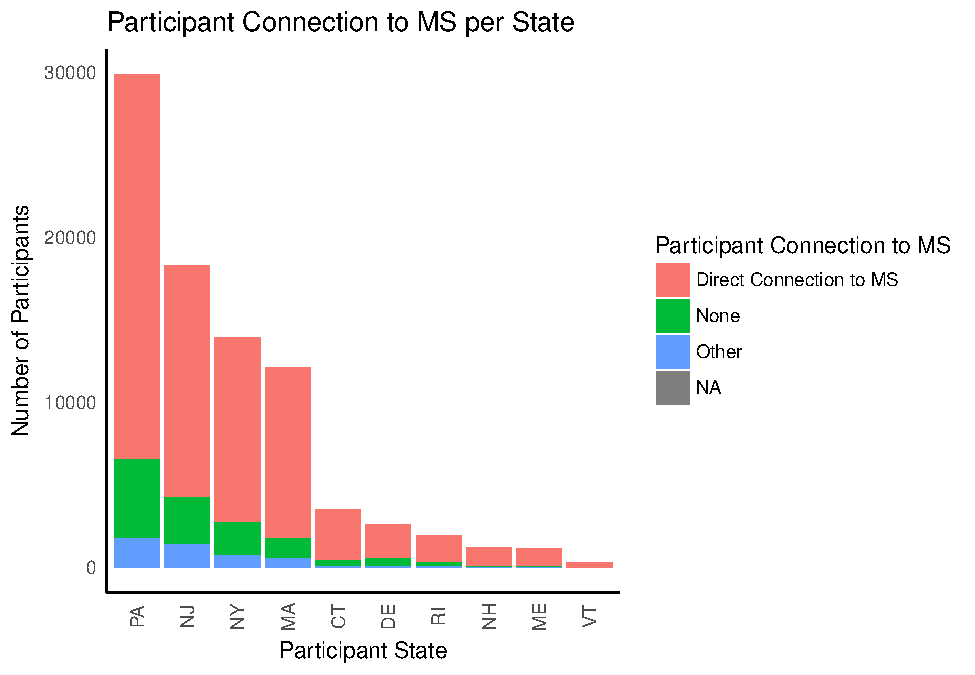
\includegraphics{index_files/figure-latex/ms.connect-1.pdf}

\begin{Shaded}
\begin{Highlighting}[]
\NormalTok{connect.ms.state <-}\StringTok{ }\NormalTok{connect.ms.state[}\KeywordTok{complete.cases}\NormalTok{(connect.ms.state), }
\NormalTok{    ]}

\NormalTok{connection.viz <-}\StringTok{ }\KeywordTok{ggplot}\NormalTok{(connect.ms.state, }\KeywordTok{aes}\NormalTok{(}\DataTypeTok{x =} \KeywordTok{reorder}\NormalTok{(connect.ms.state}\OperatorTok{$}\StringTok{`}\DataTypeTok{Address  -  Participant State/Province}\StringTok{`}\NormalTok{, }
    \OperatorTok{-}\NormalTok{n), }\DataTypeTok{y =}\NormalTok{ n, }\DataTypeTok{fill =} \StringTok{`}\DataTypeTok{Participant Connection to MS}\StringTok{`}\NormalTok{)) }\OperatorTok{+}\StringTok{ }\KeywordTok{geom_bar}\NormalTok{(}\DataTypeTok{stat =} \StringTok{"identity"}\NormalTok{)}
\NormalTok{connection.viz }\OperatorTok{+}\StringTok{ }\KeywordTok{theme_minimal}\NormalTok{() }\OperatorTok{+}\StringTok{ }\KeywordTok{theme}\NormalTok{(}\DataTypeTok{axis.text.x =} \KeywordTok{element_text}\NormalTok{(}\DataTypeTok{angle =} \DecValTok{90}\NormalTok{, }
    \DataTypeTok{vjust =} \FloatTok{0.5}\NormalTok{)) }\OperatorTok{+}\StringTok{ }\KeywordTok{labs}\NormalTok{(}\DataTypeTok{y =} \StringTok{"Number of Participants"}\NormalTok{, }\DataTypeTok{x =} \StringTok{"Participant State"}\NormalTok{, }
    \DataTypeTok{title =} \StringTok{"Participant Connection to MS per State"}\NormalTok{) }\OperatorTok{+}\StringTok{ }\KeywordTok{theme}\NormalTok{(}\DataTypeTok{panel.border =} \KeywordTok{element_blank}\NormalTok{(), }
    \DataTypeTok{panel.grid.major =} \KeywordTok{element_blank}\NormalTok{(), }\DataTypeTok{panel.grid.minor =} \KeywordTok{element_blank}\NormalTok{(), }
    \DataTypeTok{axis.line =} \KeywordTok{element_line}\NormalTok{(}\DataTypeTok{colour =} \StringTok{"black"}\NormalTok{))}
\end{Highlighting}
\end{Shaded}

\begin{figure}
\centering
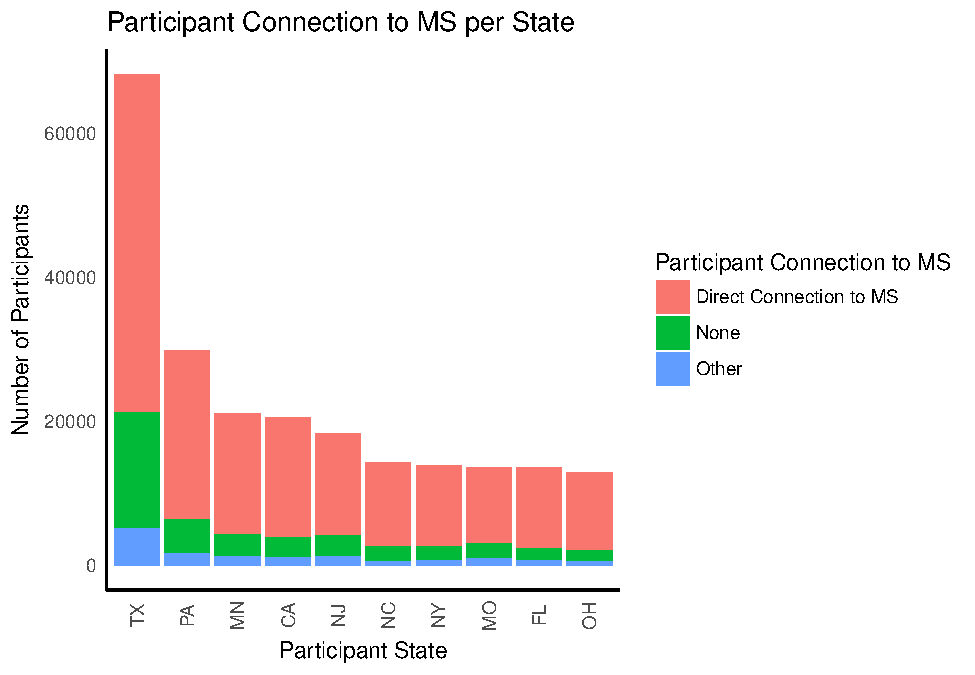
\includegraphics{index_files/figure-latex/connect.viz-1.pdf}
\caption{In the most popular states, there are consistently high numbers
of participants with direct connections to MS}
\end{figure}

We already know that on average individuals with the highest risk of
developing MS are women in the Eastern Region of the United States.
Knowing that on average participants have a personal connection to MS,
encouraging populations where prevalence is high can actually make a
difference. Understanding and building out a profile for the average
participant can prove to be valuable - let's take a look at some general
stats about our riders starting with where the majority of participants
are coming from.

\begin{Shaded}
\begin{Highlighting}[]
\NormalTok{tree.city <-}\StringTok{ }\KeywordTok{ggplot}\NormalTok{(top.city, }\KeywordTok{aes}\NormalTok{(}\DataTypeTok{area =}\NormalTok{ Count, }\DataTypeTok{fill =}\NormalTok{ Count, }
    \DataTypeTok{label =}\NormalTok{ City)) }\OperatorTok{+}\StringTok{ }\KeywordTok{geom_treemap}\NormalTok{() }\OperatorTok{+}\StringTok{ }\KeywordTok{geom_treemap_text}\NormalTok{(}\DataTypeTok{fontface =} \StringTok{"italic"}\NormalTok{, }
    \DataTypeTok{colour =} \StringTok{"white"}\NormalTok{, }\DataTypeTok{place =} \StringTok{"centre"}\NormalTok{, }\DataTypeTok{grow =} \OtherTok{TRUE}\NormalTok{)}
\NormalTok{tree.city}
\end{Highlighting}
\end{Shaded}

\begin{figure}
\centering
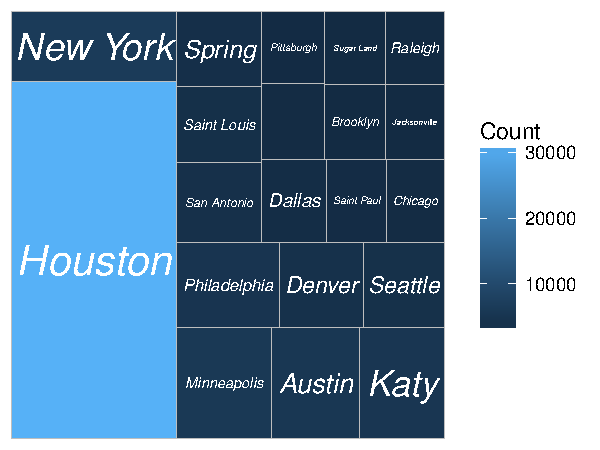
\includegraphics{index_files/figure-latex/tree-1.pdf}
\caption{Tree map of where the most participants are coming from (the
city map).}
\end{figure}

\begin{Shaded}
\begin{Highlighting}[]
\NormalTok{tree.state <-}\StringTok{ }\KeywordTok{ggplot}\NormalTok{(top.state, }\KeywordTok{aes}\NormalTok{(}\DataTypeTok{area =}\NormalTok{ Count, }\DataTypeTok{fill =}\NormalTok{ Count, }
    \DataTypeTok{label =}\NormalTok{ State)) }\OperatorTok{+}\StringTok{ }\KeywordTok{geom_treemap}\NormalTok{() }\OperatorTok{+}\StringTok{ }\KeywordTok{geom_treemap_text}\NormalTok{(}\DataTypeTok{fontface =} \StringTok{"italic"}\NormalTok{, }
    \DataTypeTok{colour =} \StringTok{"white"}\NormalTok{, }\DataTypeTok{place =} \StringTok{"centre"}\NormalTok{, }\DataTypeTok{grow =} \OtherTok{TRUE}\NormalTok{)}
\NormalTok{tree.state}
\end{Highlighting}
\end{Shaded}

\begin{figure}
\centering
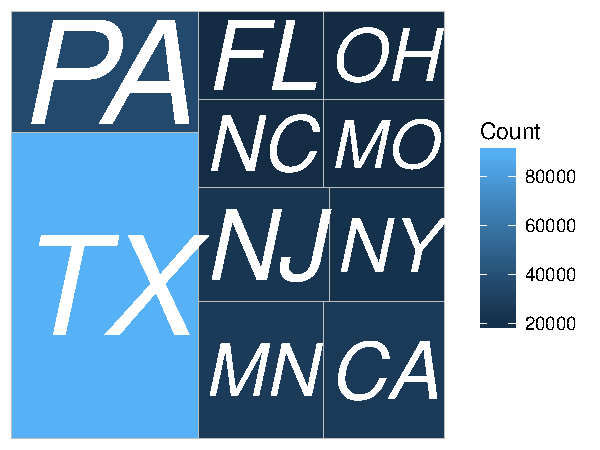
\includegraphics{index_files/figure-latex/tree-2.pdf}
\caption{Tree map of where the most participants are coming from (the
state map).}
\end{figure}

Let's compare MS prevalence with the tree maps above to quickly see if
we are on track with our assumption that where MS prevalence is high, we
will see great participation.

\begin{figure}
\centering
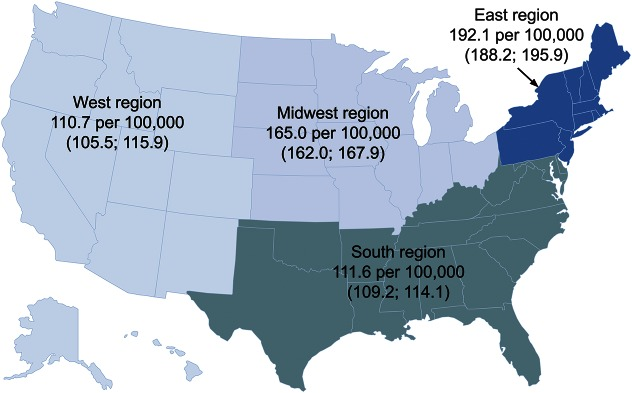
\includegraphics{RegionalMSprev.jpg}
\caption{Regional MS Prevalence}
\end{figure}

Just as we suspected, 3 out of the top 10 participant states are within
the highest prevalence region. There is a large gender gap in MS
prevalence and participation in Bike MS events, but let's take a look at
the hard numbers.

\begin{Shaded}
\begin{Highlighting}[]
\CommentTok{# make a data frame of gender counts to make visualizing}
\CommentTok{# easier}
\NormalTok{gender.df <-}\StringTok{ }\KeywordTok{as.data.frame}\NormalTok{(}\KeywordTok{table}\NormalTok{(participants}\OperatorTok{$}\StringTok{`}\DataTypeTok{Participant Gender}\StringTok{`}\NormalTok{))}
\KeywordTok{colnames}\NormalTok{(gender.df) <-}\StringTok{ }\KeywordTok{c}\NormalTok{(}\StringTok{"Gender"}\NormalTok{, }\StringTok{"Count"}\NormalTok{)}
\NormalTok{gender.overall <-}\StringTok{ }\KeywordTok{kable}\NormalTok{(gender.df, }\DataTypeTok{caption =} \StringTok{"Participant gender over all years"}\NormalTok{)}

\CommentTok{# visualize gender counts}
\NormalTok{gender.viz <-}\StringTok{ }\KeywordTok{ggplot}\NormalTok{(gender.df, }\KeywordTok{aes}\NormalTok{(}\DataTypeTok{x =}\NormalTok{ Gender, }\DataTypeTok{y =}\NormalTok{ Count, }\DataTypeTok{fill =}\NormalTok{ Gender)) }\OperatorTok{+}\StringTok{ }
\StringTok{    }\KeywordTok{geom_bar}\NormalTok{(}\DataTypeTok{stat =} \StringTok{"identity"}\NormalTok{)}
\NormalTok{gender.viz }\OperatorTok{+}\StringTok{ }\KeywordTok{theme_minimal}\NormalTok{() }\OperatorTok{+}\StringTok{ }\KeywordTok{labs}\NormalTok{(}\DataTypeTok{x =} \StringTok{"Gender"}\NormalTok{, }\DataTypeTok{y =} \StringTok{"Number of Participants"}\NormalTok{, }
    \DataTypeTok{title =} \StringTok{"Gender of Participants"}\NormalTok{) }\OperatorTok{+}\StringTok{ }\KeywordTok{scale_y_continuous}\NormalTok{(}\DataTypeTok{labels =} \KeywordTok{c}\NormalTok{(}\StringTok{"0"}\NormalTok{, }
    \StringTok{"100,000"}\NormalTok{, }\StringTok{"200,000"}\NormalTok{, }\StringTok{"300,000"}\NormalTok{)) }\OperatorTok{+}\StringTok{ }\KeywordTok{theme}\NormalTok{(}\DataTypeTok{panel.border =} \KeywordTok{element_blank}\NormalTok{(), }
    \DataTypeTok{panel.grid.major =} \KeywordTok{element_blank}\NormalTok{(), }\DataTypeTok{panel.grid.minor =} \KeywordTok{element_blank}\NormalTok{(), }
    \DataTypeTok{axis.line =} \KeywordTok{element_line}\NormalTok{(}\DataTypeTok{colour =} \StringTok{"black"}\NormalTok{))}
\NormalTok{gender.overall}
\end{Highlighting}
\end{Shaded}

\begin{longtable}[]{@{}lr@{}}
\caption{Participant gender over all years}\tabularnewline
\toprule
Gender & Count\tabularnewline
\midrule
\endfirsthead
\toprule
Gender & Count\tabularnewline
\midrule
\endhead
Male & 287795\tabularnewline
Female & 156488\tabularnewline
\bottomrule
\end{longtable}

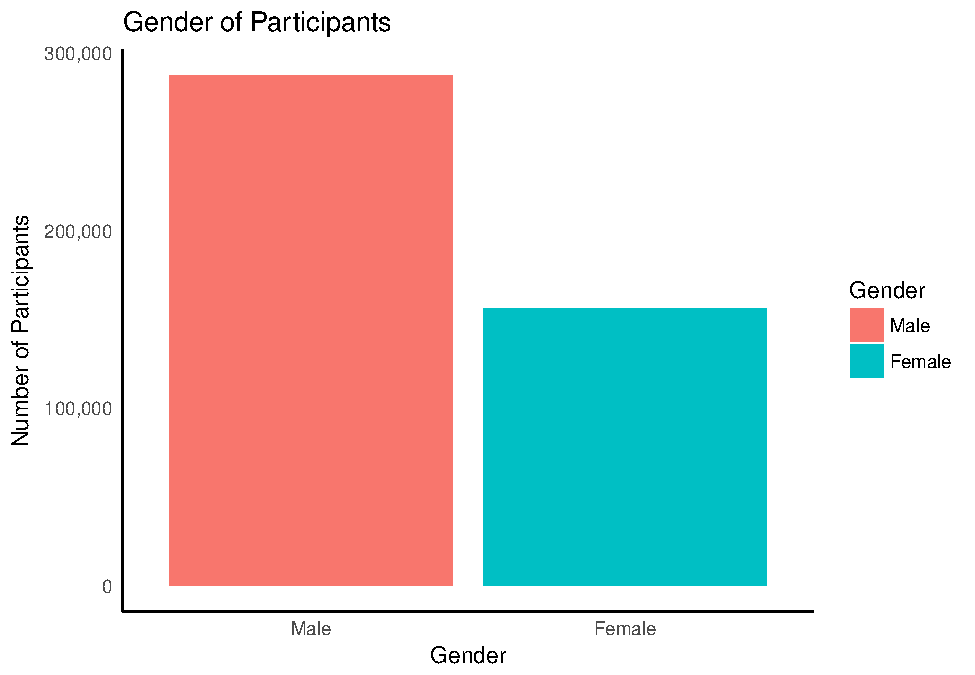
\includegraphics{index_files/figure-latex/gender.ov-1.pdf}

\begin{Shaded}
\begin{Highlighting}[]
\NormalTok{gender.k <-}\StringTok{ }\KeywordTok{kable}\NormalTok{(gender.y, }\DataTypeTok{caption =} \StringTok{"Participant gender since 2013"}\NormalTok{)}
\NormalTok{g.year.viz <-}\StringTok{ }\KeywordTok{ggplot}\NormalTok{(}\DataTypeTok{data =}\NormalTok{ gender.year, }\KeywordTok{aes}\NormalTok{(}\DataTypeTok{x =}\NormalTok{ Year, }\DataTypeTok{y =}\NormalTok{ Count, }
    \DataTypeTok{fill =}\NormalTok{ Gender)) }\OperatorTok{+}\StringTok{ }\KeywordTok{geom_bar}\NormalTok{(}\DataTypeTok{stat =} \StringTok{"identity"}\NormalTok{, }\DataTypeTok{position =} \StringTok{"dodge"}\NormalTok{)}
\NormalTok{g.year.viz }\OperatorTok{+}\StringTok{ }\KeywordTok{theme_minimal}\NormalTok{() }\OperatorTok{+}\StringTok{ }\KeywordTok{theme}\NormalTok{(}\DataTypeTok{panel.border =} \KeywordTok{element_blank}\NormalTok{(), }
    \DataTypeTok{panel.grid.major =} \KeywordTok{element_blank}\NormalTok{(), }\DataTypeTok{panel.grid.minor =} \KeywordTok{element_blank}\NormalTok{(), }
    \DataTypeTok{axis.line =} \KeywordTok{element_line}\NormalTok{(}\DataTypeTok{colour =} \StringTok{"black"}\NormalTok{)) }\OperatorTok{+}\StringTok{ }\KeywordTok{labs}\NormalTok{(}\DataTypeTok{title =} \StringTok{"Annual Participant Gender Count"}\NormalTok{) }\OperatorTok{+}\StringTok{ }
\StringTok{    }\KeywordTok{labs}\NormalTok{(}\DataTypeTok{x =} \StringTok{"Event Year"}\NormalTok{) }\OperatorTok{+}\StringTok{ }\KeywordTok{labs}\NormalTok{(}\DataTypeTok{y =} \StringTok{"Count"}\NormalTok{)}
\NormalTok{gender.k}
\end{Highlighting}
\end{Shaded}

\begin{longtable}[]{@{}lrrrrr@{}}
\caption{Participant gender since 2013}\tabularnewline
\toprule
Gender & 2013 & 2014 & 2015 & 2016 & 2017\tabularnewline
\midrule
\endfirsthead
\toprule
Gender & 2013 & 2014 & 2015 & 2016 & 2017\tabularnewline
\midrule
\endhead
Male & 67008 & 63082 & 58553 & 51641 & 47587\tabularnewline
Female & 36241 & 34643 & 32301 & 28212 & 25112\tabularnewline
\bottomrule
\end{longtable}

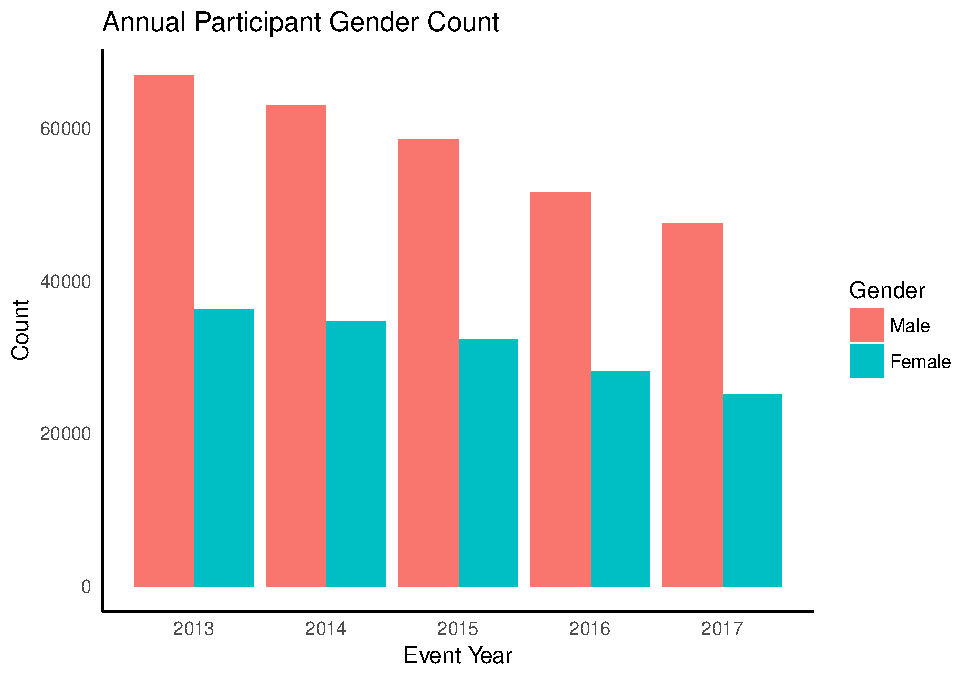
\includegraphics{index_files/figure-latex/gender.sum-1.pdf}

Just as Bike MS had briefed us, the average participant is male. Maybe
we assume that, in general, more men than women cycle. However, in 2015
PeopleforBikes.org conducted a U.S. Bicycling Participation Survey and
found that from a sample of 16,000 citizens 43\% of women reported
participating in cycling activities. Bike MS is missing out on targeting
the female demographic, which also happens to have the highest
prevalence and incidence of MS. Is there a particular industry women
contribute to most in the workforce?

\begin{longtable}[]{@{}lrrrrr@{}}
\caption{Top 10 Reported Occupations of Female
Participants}\tabularnewline
\toprule
Participant Occupation & 2013 & 2014 & 2015 & 2016 & 2017\tabularnewline
\midrule
\endfirsthead
\toprule
Participant Occupation & 2013 & 2014 & 2015 & 2016 & 2017\tabularnewline
\midrule
\endhead
Healthcare & 2251 & 2074 & 1888 & 1525 & 1305\tabularnewline
Education and Training & 1212 & 1160 & 1092 & 815 & 701\tabularnewline
Accounting & 674 & 644 & 604 & 447 & 419\tabularnewline
Student & 516 & 445 & 434 & 287 & 242\tabularnewline
Sales & 510 & 474 & 429 & 342 & 273\tabularnewline
Engineering & 457 & 497 & 504 & 319 & 260\tabularnewline
Information Technology (IT) & 410 & 383 & 371 & 297 & 267\tabularnewline
Legal and Paralegal & 397 & 399 & 364 & 248 & 206\tabularnewline
Marketing & 385 & 413 & 375 & 266 & 223\tabularnewline
Executive/Management & 343 & 332 & 299 & 247 & 209\tabularnewline
\bottomrule
\end{longtable}

It appears women have the highest number of cyclists working in the
healthcare industry. There is a common theme that connects each of the
first priority business questions, which is generated by addressing
greatest growth opportunities for corporate teams. Furthermore, our
recommendation is to target corporations located in the East Coast
specifically those operating in the healthcare sector. According to
Business Insider, in 22 states Walmart is the largest employer, many of
which are within easy travel distance from the most successful Bike MS
events. More importantly, six out of the ten states defined as Eastern
Region (highest overall MS prevalence) have Healthcare listed as its
largest employer - Pennsylvania, Vermont, Rhode Island, Massachusetts,
Connecticut, and Delaware. Can we tell if healthcare is represented in
the Eastern Region?

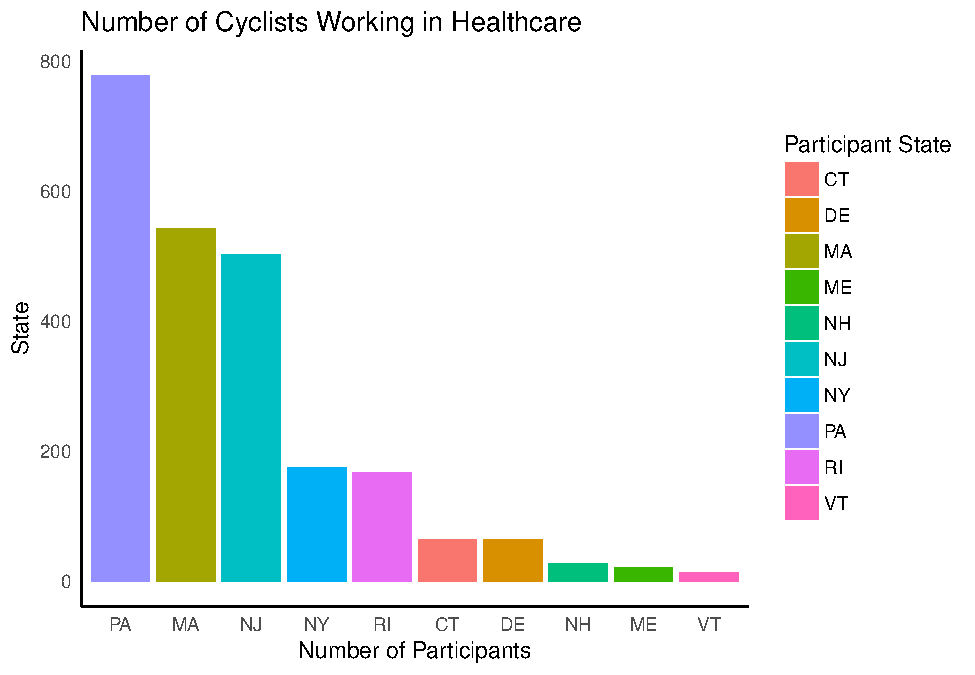
\includegraphics{index_files/figure-latex/east.health-1.pdf}

The data shows us that only three of the six states who have Healthcare
listed as their largest employer have large numbers of cyclists signing
up for Bike MS events. In past years these numbers were higher, but have
been steadily declining. Of the top states that participants record as
their home state, all of the major occupational industries are
declining.

\begin{Shaded}
\begin{Highlighting}[]
\KeywordTok{ggplot}\NormalTok{(state.occ) }\OperatorTok{+}\StringTok{ }
\KeywordTok{geom_point}\NormalTok{(}\KeywordTok{aes}\NormalTok{(}\DataTypeTok{x =} \StringTok{`}\DataTypeTok{Fiscal Year}\StringTok{`}\NormalTok{, }\DataTypeTok{y =}\NormalTok{ n, }\DataTypeTok{colour =} \StringTok{`}\DataTypeTok{Participant Occupation}\StringTok{`}\NormalTok{)) }\OperatorTok{+}\StringTok{ }
\StringTok{    }\KeywordTok{geom_path}\NormalTok{(}\KeywordTok{aes}\NormalTok{(}\DataTypeTok{x =} \StringTok{`}\DataTypeTok{Fiscal Year}\StringTok{`}\NormalTok{, }\DataTypeTok{y =}\NormalTok{ n, }\DataTypeTok{colour =} \StringTok{`}\DataTypeTok{Participant Occupation}\StringTok{`}\NormalTok{)) }\OperatorTok{+}\StringTok{ }
\StringTok{    }\KeywordTok{facet_wrap}\NormalTok{(}\OperatorTok{~}\StringTok{`}\DataTypeTok{Address - Participant State}\StringTok{`}\NormalTok{, }\DataTypeTok{scales =} \StringTok{"free_y"}\NormalTok{, }
        \DataTypeTok{nrow =} \DecValTok{2}\NormalTok{) }\OperatorTok{+}\StringTok{ }
\KeywordTok{theme_pander}\NormalTok{() }\OperatorTok{+}\StringTok{ }\KeywordTok{theme}\NormalTok{(}\DataTypeTok{legend.position =} \StringTok{"right"}\NormalTok{) }\OperatorTok{+}\StringTok{ }\KeywordTok{theme}\NormalTok{(}\DataTypeTok{axis.text.x =} \KeywordTok{element_text}\NormalTok{(}\DataTypeTok{angle =} \DecValTok{90}\NormalTok{, }
    \DataTypeTok{vjust =} \FloatTok{0.5}\NormalTok{)) }\OperatorTok{+}\StringTok{ }\KeywordTok{labs}\NormalTok{(}\DataTypeTok{x =} \StringTok{"Year"}\NormalTok{, }\DataTypeTok{y =} \StringTok{"Number of Participants"}\NormalTok{)}
\end{Highlighting}
\end{Shaded}

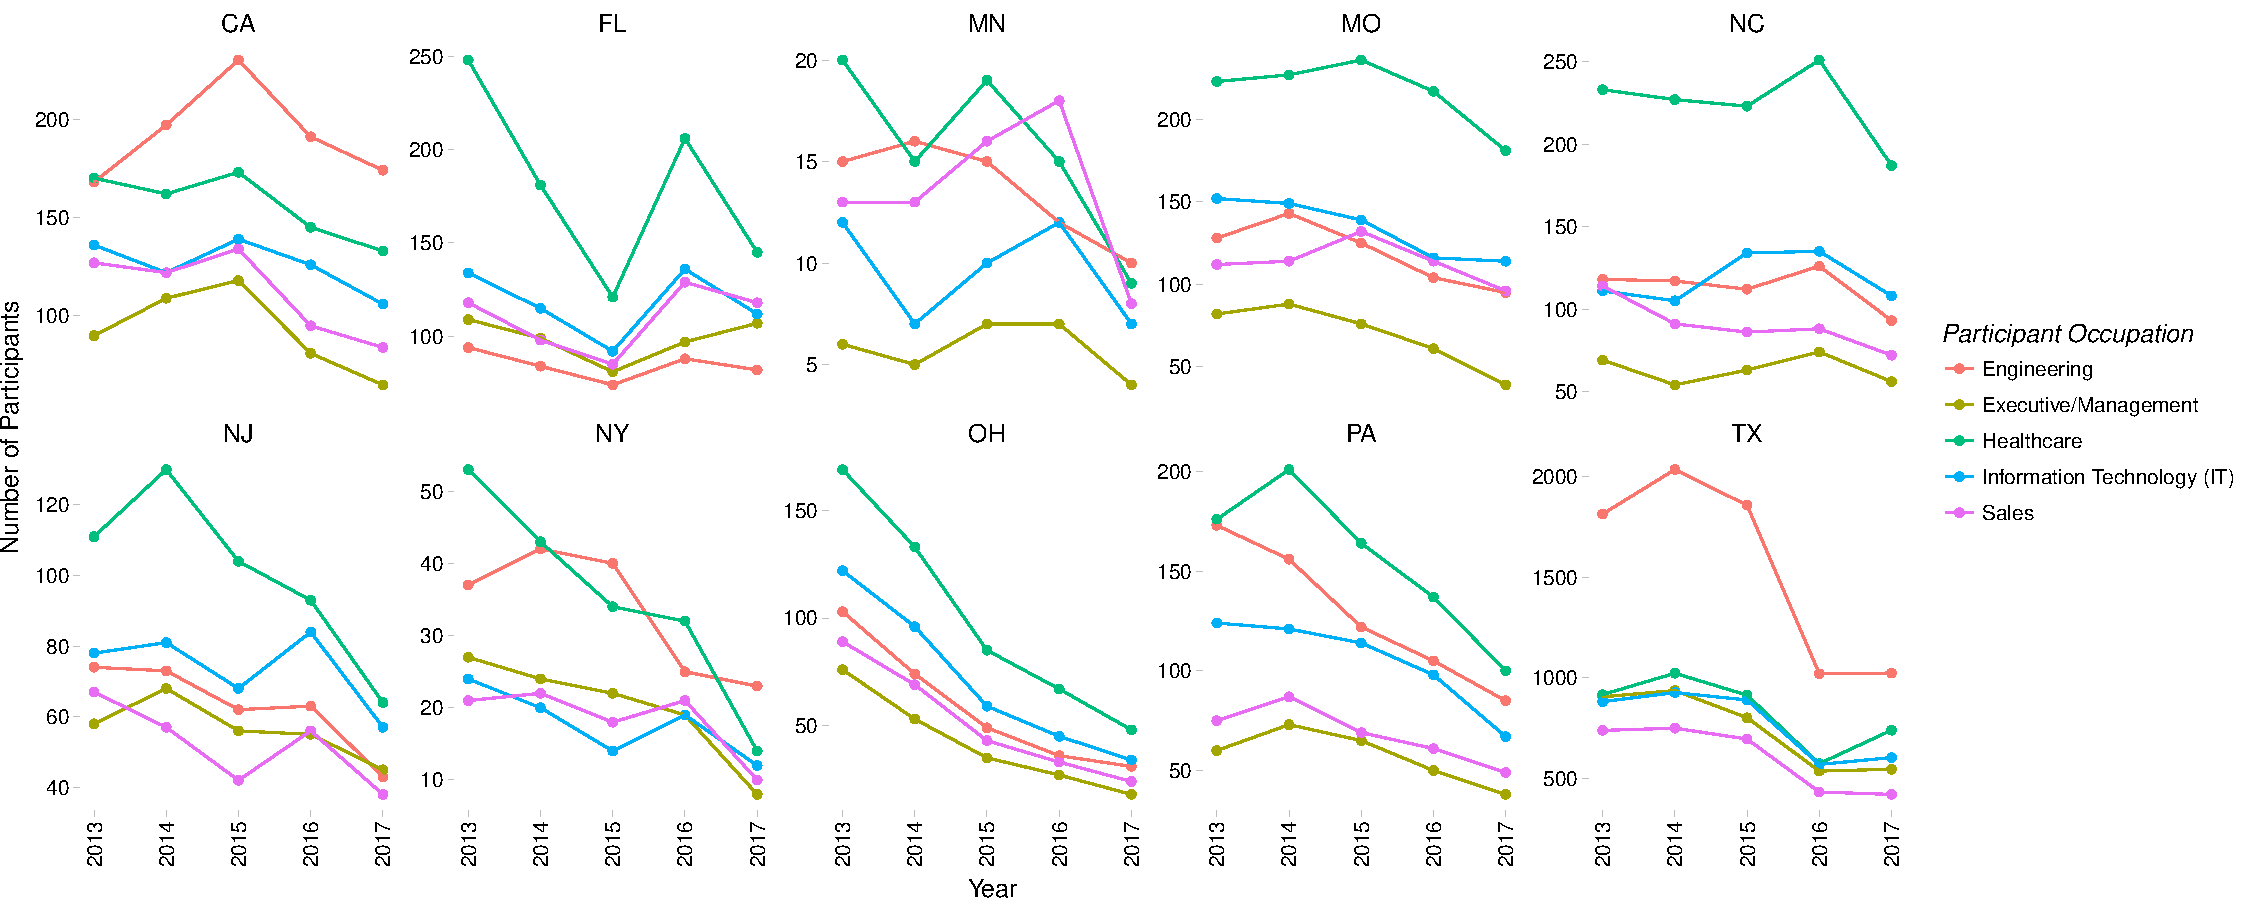
\includegraphics{index_files/figure-latex/facet.participants-1.pdf}

\begin{Shaded}
\begin{Highlighting}[]
\NormalTok{occupation.state <-}\StringTok{ }\NormalTok{participants}
\NormalTok{occupation.state}\OperatorTok{$}\StringTok{`}\DataTypeTok{Address  -  Participant State/Province}\StringTok{`}\NormalTok{ <-}\StringTok{ }\KeywordTok{as.factor}\NormalTok{(occupation.state}\OperatorTok{$}\StringTok{`}\DataTypeTok{Address  -  Participant State/Province}\StringTok{`}\NormalTok{)}
\NormalTok{healthcare <-}\StringTok{ }\NormalTok{occupation.state }\OperatorTok\StringTok{ }\KeywordTok{select}\NormalTok{(}\KeywordTok{everything}\NormalTok{()) }\OperatorTok\StringTok{ }\KeywordTok{filter}\NormalTok{(}\StringTok{`}\DataTypeTok{Participant Occupation}\StringTok{`} \OperatorTok{==}\StringTok{ }
\StringTok{    "Healthcare"}\NormalTok{) }\OperatorTok\StringTok{ }\KeywordTok{group_by}\NormalTok{(}\StringTok{`}\DataTypeTok{Address  -  Participant State/Province}\StringTok{`}\NormalTok{) }\OperatorTok\StringTok{ }
\StringTok{    }\KeywordTok{tally}\NormalTok{() }\OperatorTok\StringTok{ }\KeywordTok{arrange}\NormalTok{(}\KeywordTok{desc}\NormalTok{(n)) }\OperatorTok\StringTok{ }\KeywordTok{top_n}\NormalTok{(}\DecValTok{10}\NormalTok{)}
\end{Highlighting}
\end{Shaded}

\hypertarget{can-we-apply-those-opportunities-to-specific-ridesmarkets-especially-our-biggest-events}{%
\subsection{Can we apply those opportunities to specific rides/markets,
especially our biggest
events?}\label{can-we-apply-those-opportunities-to-specific-ridesmarkets-especially-our-biggest-events}}

Bike MS has supplied us with budget information for their top 20 events.
Three out of the top 20 events are located in the Eastern region where
we are recommending Bike MS focus their marketing/advertising efforts.
Concentration of events and date of event are of particular interest,
because we will saturate the market with too many events in one area
especially if they are only a couple months apart.

\begin{Shaded}
\begin{Highlighting}[]
\NormalTok{states <-}\StringTok{ }\KeywordTok{map_data}\NormalTok{(}\StringTok{"state"}\NormalTok{)}
\NormalTok{gg <-}\StringTok{ }\KeywordTok{ggplot}\NormalTok{()}
\NormalTok{gg <-}\StringTok{ }\NormalTok{gg }\OperatorTok{+}\StringTok{ }\KeywordTok{geom_map}\NormalTok{(}\DataTypeTok{data =}\NormalTok{ states, }\DataTypeTok{map =}\NormalTok{ states, }\KeywordTok{aes}\NormalTok{(}\DataTypeTok{x =}\NormalTok{ long, }
    \DataTypeTok{y =}\NormalTok{ lat, }\DataTypeTok{map_id =}\NormalTok{ region), }\DataTypeTok{color =} \StringTok{"white"}\NormalTok{, }\DataTypeTok{fill =} \StringTok{"#cccccc"}\NormalTok{, }
    \DataTypeTok{size =} \FloatTok{0.5}\NormalTok{)}
\NormalTok{gg <-}\StringTok{ }\NormalTok{gg }\OperatorTok{+}\StringTok{ }\KeywordTok{geom_point}\NormalTok{(}\DataTypeTok{data =} \KeywordTok{arrange}\NormalTok{(topEvents18, }\KeywordTok{desc}\NormalTok{(topEvents18}\OperatorTok{$}\NormalTok{Budget)), }
    \KeywordTok{aes}\NormalTok{(}\DataTypeTok{x =}\NormalTok{ topEvents18}\OperatorTok{$}\NormalTok{Lon, }\DataTypeTok{y =}\NormalTok{ topEvents18}\OperatorTok{$}\NormalTok{Lat, }\DataTypeTok{size =}\NormalTok{ topEvents18}\OperatorTok{$}\NormalTok{Budget), }
    \DataTypeTok{shape =} \DecValTok{21}\NormalTok{, }\DataTypeTok{color =} \StringTok{"white"}\NormalTok{, }\DataTypeTok{fill =} \StringTok{"steelblue"}\NormalTok{)}
\NormalTok{gg <-}\StringTok{ }\NormalTok{gg }\OperatorTok{+}\StringTok{ }\KeywordTok{geom_map}\NormalTok{(}\DataTypeTok{data =}\NormalTok{ vor_df, }\DataTypeTok{map =}\NormalTok{ vor_df, }\KeywordTok{aes}\NormalTok{(}\DataTypeTok{x =}\NormalTok{ long, }
    \DataTypeTok{y =}\NormalTok{ lat, }\DataTypeTok{map_id =}\NormalTok{ id), }\DataTypeTok{color =} \StringTok{"#a5a5a5"}\NormalTok{, }\DataTypeTok{fill =} \StringTok{"#FFFFFF00"}\NormalTok{, }
    \DataTypeTok{size =} \FloatTok{0.5}\NormalTok{)}
\NormalTok{gg <-}\StringTok{ }\NormalTok{gg }\OperatorTok{+}\StringTok{ }\KeywordTok{scale_size}\NormalTok{(}\DataTypeTok{range =} \KeywordTok{c}\NormalTok{(}\DecValTok{2}\NormalTok{, }\DecValTok{15}\NormalTok{))}
\NormalTok{gg <-}\StringTok{ }\NormalTok{gg }\OperatorTok{+}\StringTok{ }\KeywordTok{coord_map}\NormalTok{(}\StringTok{"albers"}\NormalTok{, }\DataTypeTok{lat0 =} \DecValTok{30}\NormalTok{, }\DataTypeTok{lat1 =} \DecValTok{40}\NormalTok{)}
\NormalTok{gg <-}\StringTok{ }\NormalTok{gg }\OperatorTok{+}\StringTok{ }\KeywordTok{theme_map}\NormalTok{()}
\NormalTok{gg <-}\StringTok{ }\NormalTok{gg }\OperatorTok{+}\StringTok{ }\KeywordTok{theme}\NormalTok{(}\DataTypeTok{legend.position =} \StringTok{"none"}\NormalTok{)}
\NormalTok{gg}
\end{Highlighting}
\end{Shaded}

\begin{figure}
\centering
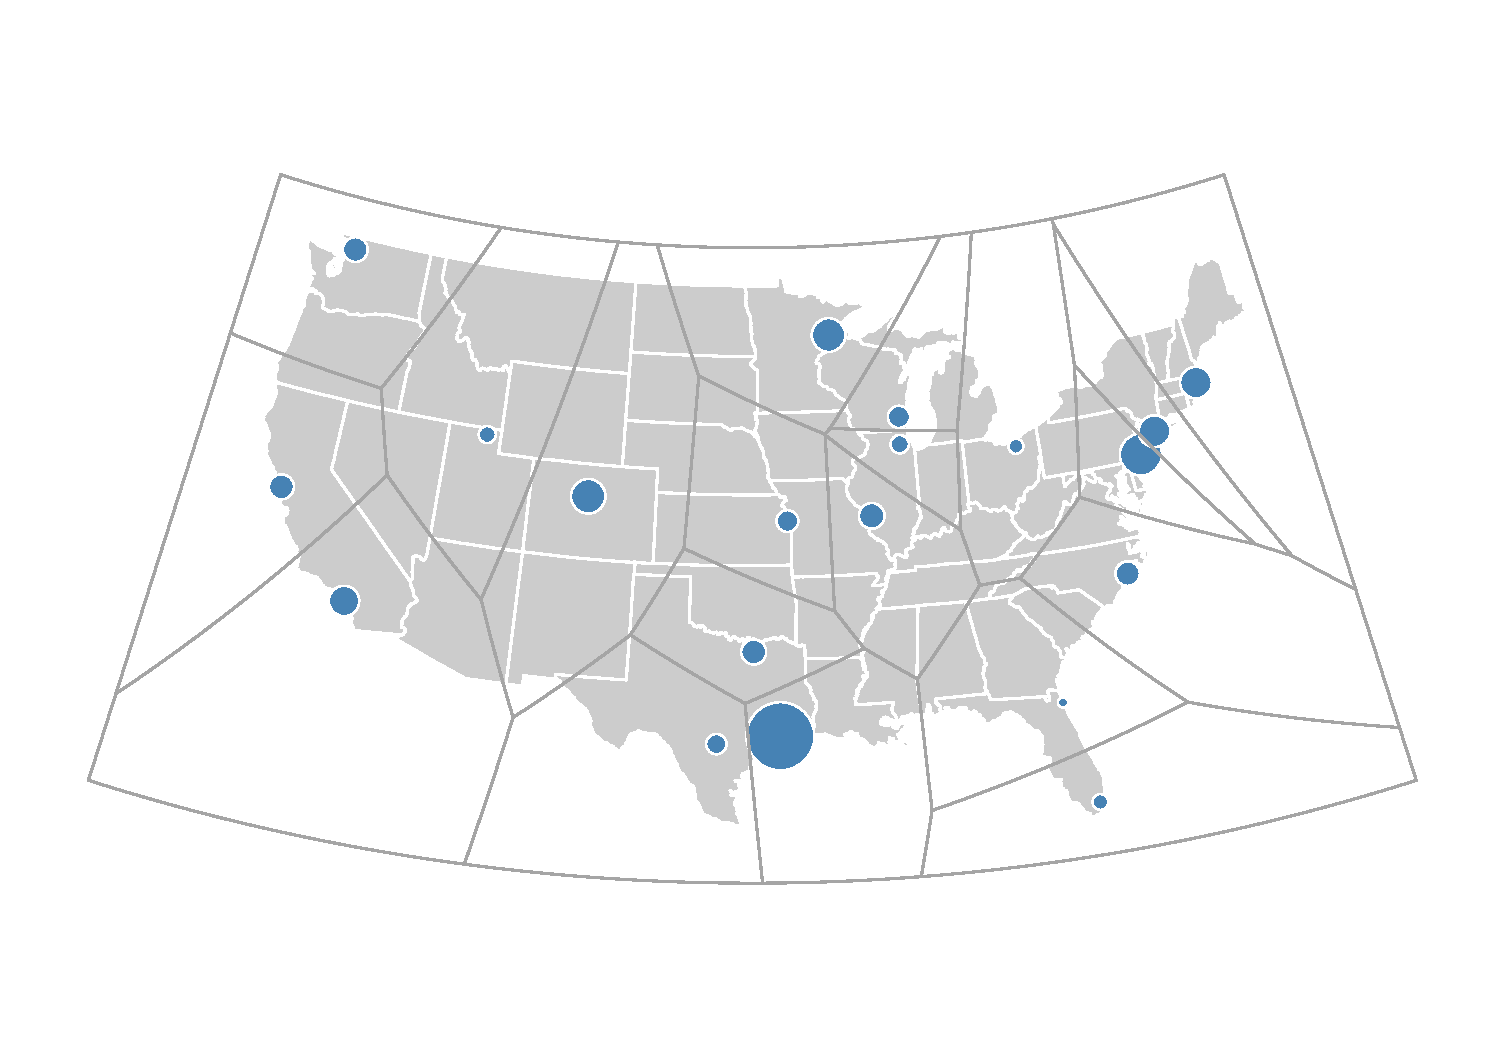
\includegraphics{index_files/figure-latex/voronoi-1.pdf}
\caption{Voronoi of Top Events for 2018}
\end{figure}

The voronoi diagram partitions the United States into regions whose
distance to the seed (in our case event) is the shortest. This allows us
to see which populations should be going to which event based on
distance from the event. Following our central theme, one practical
recommendation is to allocate resources to boost participation in the
Northeast states and in particular the states where the largest employer
is operating in healthcare. Referencing a visual shown above, we would
like to highlight the following states and encourage increased
advertising in the following states because of the low numbers of
cyclists working in healthcare. Below are top priority states with their
respective state-wide largest employer.

\begin{longtable}[]{@{}cl@{}}
\toprule
State & Employer\tabularnewline
\midrule
\endhead
Connecticut & Yale New Haven Health System\tabularnewline
Delaware & Christiana Care Health System\tabularnewline
Rhode Island & Lifespan System of Hospitals\tabularnewline
Vermont & The University of Vermont Medical Center\tabularnewline
\bottomrule
\end{longtable}

Additionally for your reference, here are the largest employers in each
state. You will also notice that Walmart is within the target region,
which would obviously be a great sponsor.

\begin{figure}
\centering
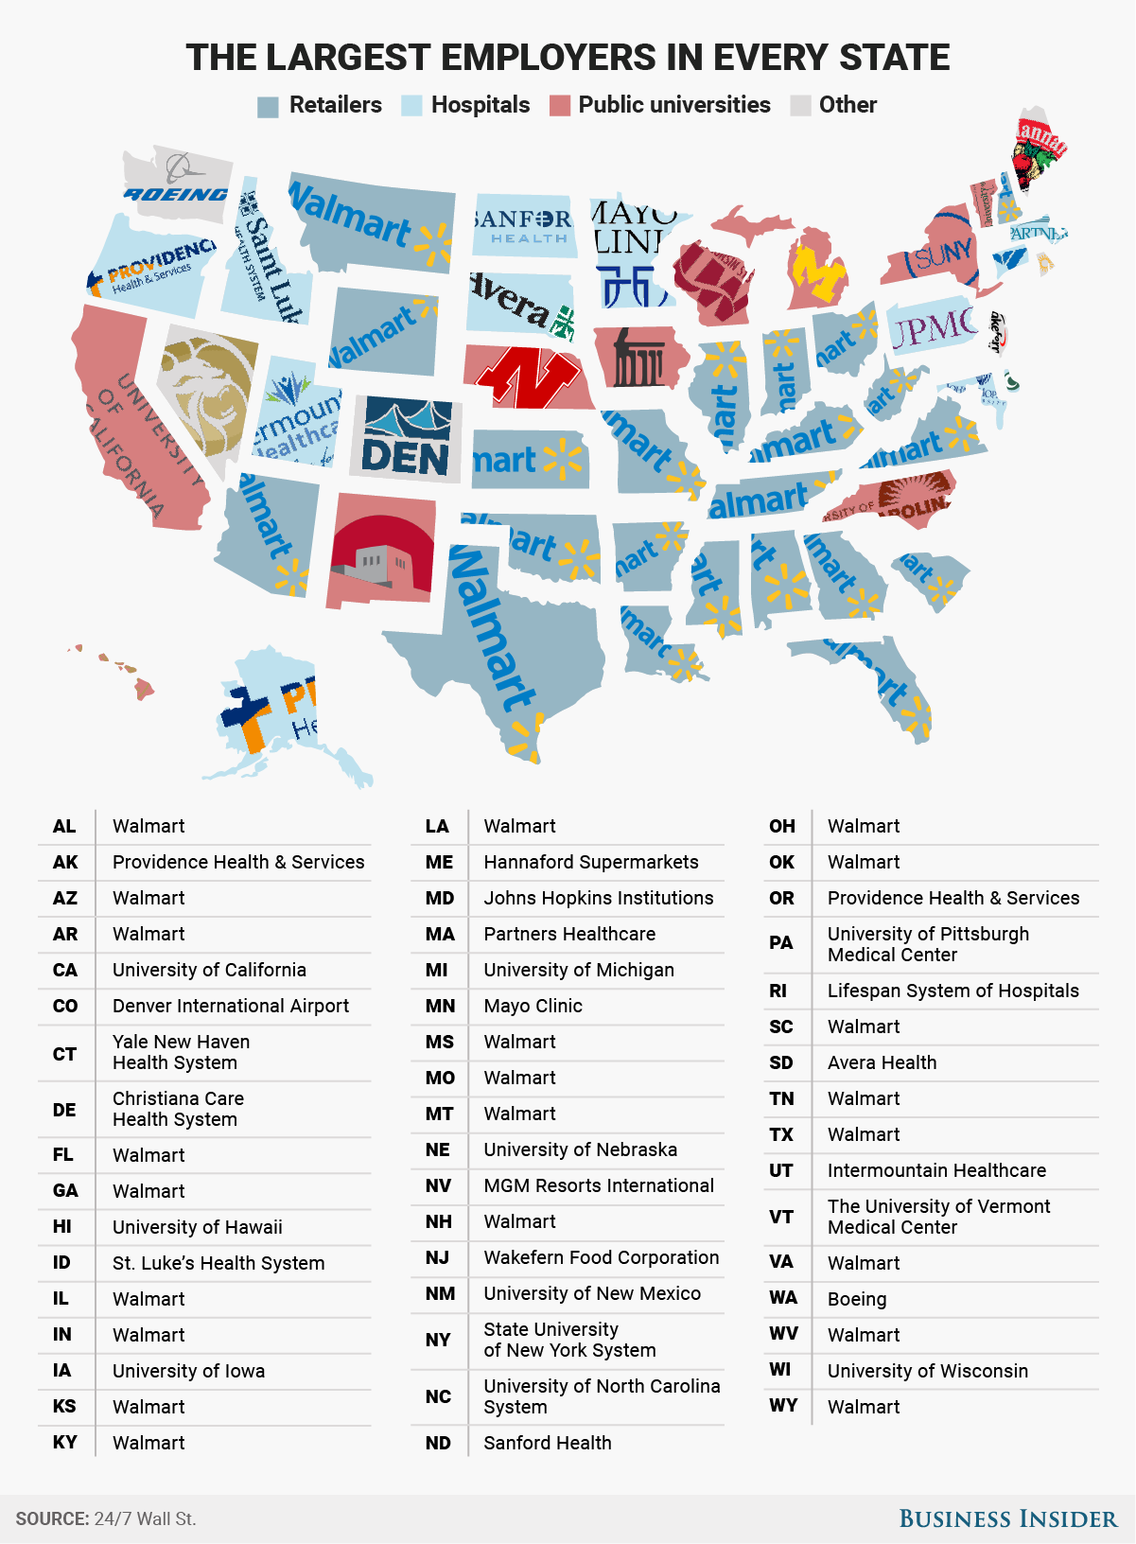
\includegraphics{BILargestEmployer.png}
\caption{Largest Employer Image}
\end{figure}

\begin{Shaded}
\begin{Highlighting}[]
\NormalTok{east.health.viz <-}\StringTok{ }\KeywordTok{ggplot}\NormalTok{(east.health, }\KeywordTok{aes}\NormalTok{(}\DataTypeTok{x =} \KeywordTok{reorder}\NormalTok{(}\StringTok{`}\DataTypeTok{Participant State}\StringTok{`}\NormalTok{, }
    \OperatorTok{-}\NormalTok{Count), }\DataTypeTok{y =}\NormalTok{ Count, }\DataTypeTok{fill =} \StringTok{`}\DataTypeTok{Participant State}\StringTok{`}\NormalTok{)) }\OperatorTok{+}\StringTok{ }\KeywordTok{geom_bar}\NormalTok{(}\DataTypeTok{stat =} \StringTok{"identity"}\NormalTok{)}
\NormalTok{east.health.viz }\OperatorTok{+}\StringTok{ }\KeywordTok{theme_minimal}\NormalTok{() }\OperatorTok{+}\StringTok{ }\KeywordTok{theme}\NormalTok{(}\DataTypeTok{panel.border =} \KeywordTok{element_blank}\NormalTok{(), }
    \DataTypeTok{panel.grid.major =} \KeywordTok{element_blank}\NormalTok{(), }\DataTypeTok{panel.grid.minor =} \KeywordTok{element_blank}\NormalTok{(), }
    \DataTypeTok{axis.line =} \KeywordTok{element_line}\NormalTok{(}\DataTypeTok{colour =} \StringTok{"black"}\NormalTok{)) }\OperatorTok{+}\StringTok{ }\KeywordTok{labs}\NormalTok{(}\DataTypeTok{x =} \StringTok{"Number of Participants"}\NormalTok{, }
    \DataTypeTok{y =} \StringTok{"State"}\NormalTok{, }\DataTypeTok{title =} \StringTok{"Number of Cyclists Working in Healthcare Within the Target Region"}\NormalTok{)}
\end{Highlighting}
\end{Shaded}

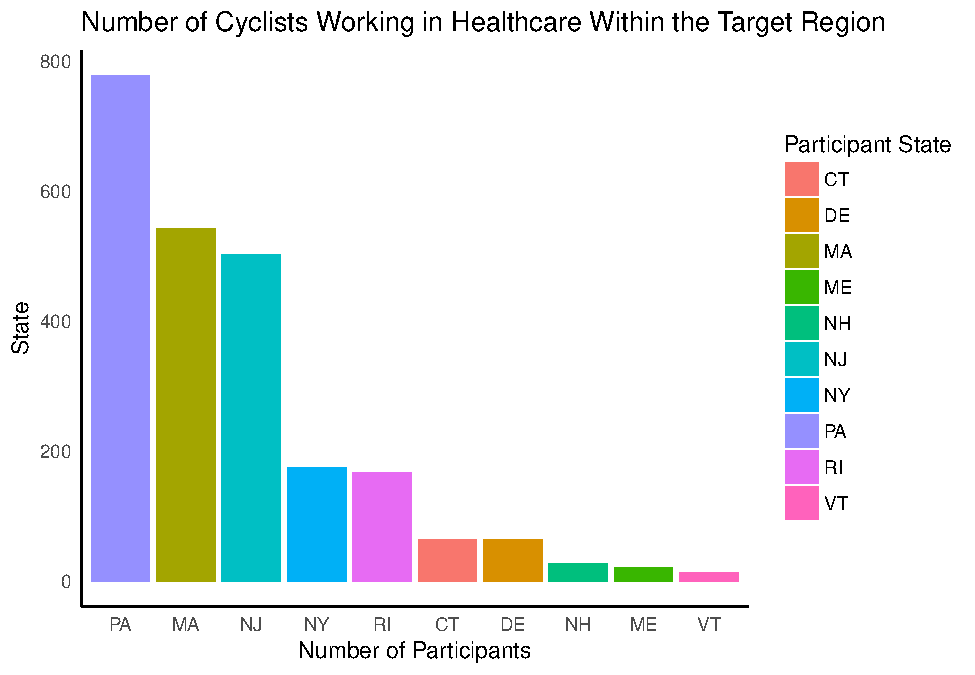
\includegraphics{index_files/figure-latex/healthy.east-1.pdf}

\hypertarget{what-industries-have-had-the-strongest-involvement-in-bike-ms-in-the-last-five-years-and-what-occupations-were-responsible-for-most-of-our-fundraising}{%
\subsection{What industries have had the strongest involvement in Bike
MS in the last five years and what occupations were responsible for most
of our
fundraising?}\label{what-industries-have-had-the-strongest-involvement-in-bike-ms-in-the-last-five-years-and-what-occupations-were-responsible-for-most-of-our-fundraising}}

Involvement with Bike MS can take two forms, either you participate as a
cyclist or you donate to the fundraiser. We have already seen that the
top occupations of participants are Engineering, Healthcare, Sales, IT,
and Executive Management. From the donations data, we can discern what
industries are the top donors.

\begin{figure}
\centering
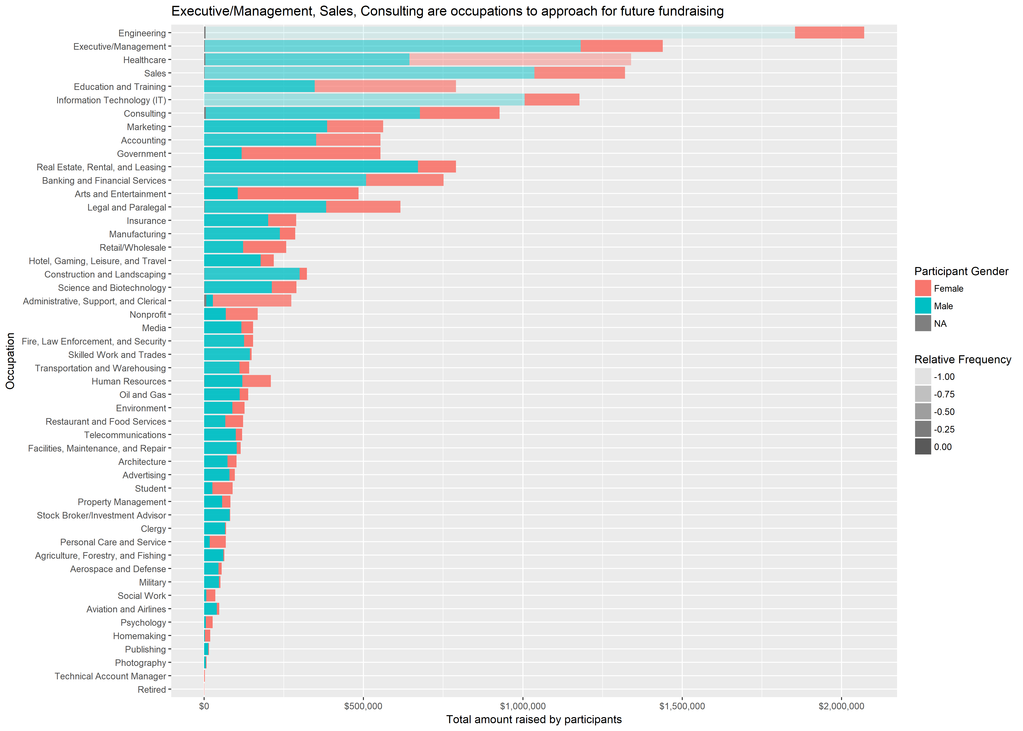
\includegraphics{topOccupationsdonation.png}
\caption{Top Donating Occupations}
\end{figure}

The data shows us that the same occupations are responsible for the
majority of the fundraising. The darker the color shows that the average
donation is Men are responsible for a large sum of money, but mainly due
to the significantly higher number of participants. The average donation
from women is just as much as men. The national teams are also
responsible for a significant amount of involvement - fundraising and
participation. Here are some statistics on the top national teams over
the years.

\begin{figure}
\centering
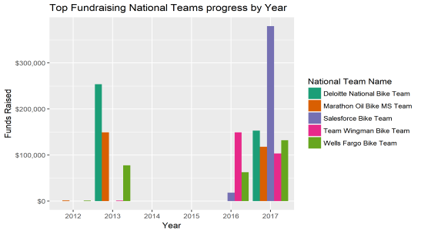
\includegraphics{nationalteams1.png}
\caption{Involvement of Top National Teams}
\end{figure}

Each of these national teams have major offices across the United States
and therefore can participate in the most popular Bike MS events. It is
reflected

\begin{figure}
\centering
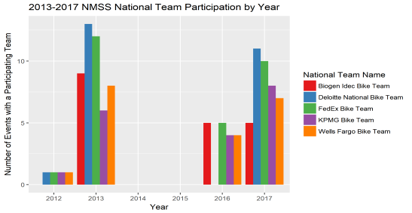
\includegraphics{nationalteams2.png}
\caption{Participation of Top National Teams}
\end{figure}

\begin{figure}
\centering
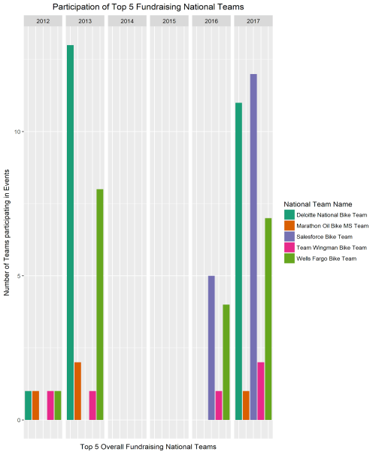
\includegraphics{nationalteams3.png}
\caption{Number of Teams per National Team}
\end{figure}

Upon exploration it was seen that the information was consistent with
the rest of the data. The National Teams with the highest amount of
revenue raised, varied from year to year during the 2013-2017 time
period. Regardless of how much it varied these National Teams are
responsible for a large portion of the overall revenue raised. Although
some National Teams tend to repeat participation a larger portion of
them do not, either way their teams tend to have more team members. The
information here was consistent with other analyses showing the
``Primary Connection to MS'' overwhelmingly as ``Friend has MS''
followed by None/NA, and ``Relative has MS''. It is important to
recommend that Bike MS definitely prioritize keeping these teams
engaged, but highlight the fact there is a lack of healthcare
organizations among this list.

\hypertarget{can-we-tie-together-these-industries-and-occupations-to-identify-gapsopportunities}{%
\subsection{Can we tie together these industries and occupations to
identify
gaps/opportunities?}\label{can-we-tie-together-these-industries-and-occupations-to-identify-gapsopportunities}}

Again, the top national teams with the most involvement are from male
dominated fields. Our central themes all apply to this question - as we
stated above there is a lack of healthcare organizations involved in
putting together formal teams. Of particular interest, are the
corporations that are spread out across the United States and those
located on the East coast. Taking a closer look at Deloitte and
Salesforce, for example in 2017, Deloitte reported employing almost
85,000 operating in 97 U.S. cities while Salesforce reported employing
25,000. Targeting companies with offices in multiple cities across the
U.S. has the potential to produce highly involved national teams.

\hypertarget{what-is-the-common-denominator-for-our-top-performing-corporate-teams}{%
\subsection{What is the common denominator for our top performing
corporate
teams?}\label{what-is-the-common-denominator-for-our-top-performing-corporate-teams}}

Echoing the previous answer, the top performing corporate teams have
employ a large population and have offices across the United States.
Returning to our central themes, the data tells us that connection to
multiple sclerosis drives participants and donors to this massive
fundraiser. The purpose of Bike MS is to fund research, advocate for
social and political change, provide education, and sponsor services
that help people with multiple sclerosis and their families. If the
prevalence and incidence numbers are true then there is no reason
participation and fundraising efforts should be declining. Let's take a
look at the biggest common denominator for not only corporate teams, but
everyone involved.

\begin{figure}
\centering
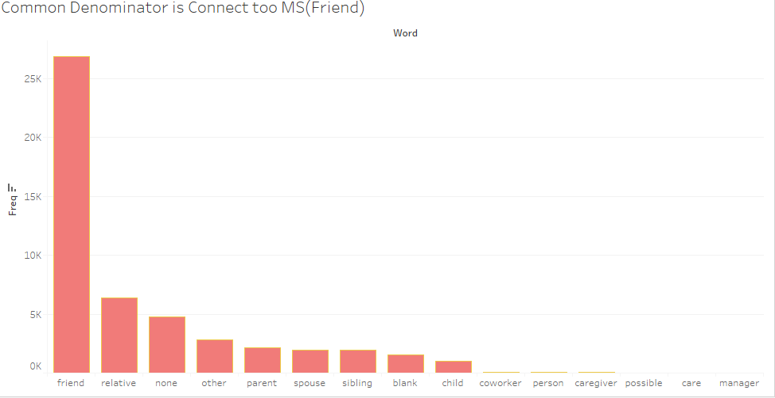
\includegraphics{commondenominator.png}
\caption{Common Denominator}
\end{figure}

Of all the responses of reported connection to MS from the corporate
teams and participants, most people have a direct connection to a friend
afflicted by MS. This finding does not come as a surprise given that the
friend category would have the widest reach compared to sibling or
spouse relationships. As participation and donations for this fundraiser
decline, the one constant is that the overall prevalence and incidence
of multiple sclerosis is something that persists. Focusing on the
populations, occupations, and geographical locations that are impacted
by this disease the most will ensure consistent fundraising and
participation. Here is a visualization of the growing MS population in
the United States that shows the magnitude of just the lives who are
living with the disease.

\begin{Shaded}
\begin{Highlighting}[]
\CommentTok{# growth of MS build dataframe of dates with weekly growth}
\CommentTok{# interval}
\NormalTok{start <-}\StringTok{ }\KeywordTok{as.Date}\NormalTok{(}\StringTok{"2012-01-01"}\NormalTok{)}
\NormalTok{end <-}\StringTok{ }\KeywordTok{as.Date}\NormalTok{(}\StringTok{"2017-01-08"}\NormalTok{)}
\NormalTok{grow.date <-}\StringTok{ }\KeywordTok{as.data.frame}\NormalTok{(}\KeywordTok{seq}\NormalTok{(start, end, }\DataTypeTok{by =} \StringTok{"1 week"}\NormalTok{))}
\NormalTok{grow.ms <-}\StringTok{ }\KeywordTok{as.data.frame}\NormalTok{(}\KeywordTok{seq}\NormalTok{(}\DataTypeTok{length =} \DecValTok{263}\NormalTok{, }\DataTypeTok{from =} \DecValTok{400001}\NormalTok{, }\DataTypeTok{by =} \FloatTok{2290.0763}\NormalTok{))}

\NormalTok{ms.growth <-}\StringTok{ }\KeywordTok{as.data.frame}\NormalTok{(}\KeywordTok{cbind}\NormalTok{(grow.date, grow.ms))}
\KeywordTok{colnames}\NormalTok{(ms.growth) <-}\StringTok{ }\KeywordTok{c}\NormalTok{(}\StringTok{"Date"}\NormalTok{, }\StringTok{"Weekly Increase"}\NormalTok{)}
\NormalTok{ms.growth <-}\StringTok{ }\NormalTok{ms.growth }\OperatorTok\StringTok{ }\KeywordTok{mutate}\NormalTok{(}\DataTypeTok{Country =} \StringTok{"United States"}\NormalTok{)}
\NormalTok{ms.growth <-}\StringTok{ }\NormalTok{ms.growth }\OperatorTok\StringTok{ }\KeywordTok{mutate}\NormalTok{(}\DataTypeTok{Longitude =} \FloatTok{37.0902}\NormalTok{) }\OperatorTok\StringTok{ }\KeywordTok{mutate}\NormalTok{(}\DataTypeTok{Latitude =} \FloatTok{95.7129}\NormalTok{) }\OperatorTok\StringTok{ }
\StringTok{    }\KeywordTok{mutate}\NormalTok{(}\DataTypeTok{ID =} \StringTok{"main"}\NormalTok{)}

\NormalTok{ms.growth}\OperatorTok{$}\StringTok{`}\DataTypeTok{Weekly Increase}\StringTok{`}\NormalTok{ <-}\StringTok{ }\KeywordTok{round}\NormalTok{(ms.growth}\OperatorTok{$}\StringTok{`}\DataTypeTok{Weekly Increase}\StringTok{`}\NormalTok{, }
    \DataTypeTok{digits =} \DecValTok{0}\NormalTok{)}

\NormalTok{usa <-}\StringTok{ }\KeywordTok{map_data}\NormalTok{(}\StringTok{"usa"}\NormalTok{)}

\NormalTok{usa.map <-}\StringTok{ }\KeywordTok{ggplot}\NormalTok{()}
\NormalTok{usa.map <-}\StringTok{ }\NormalTok{usa.map }\OperatorTok{+}\StringTok{ }\KeywordTok{geom_map}\NormalTok{(}\DataTypeTok{data =}\NormalTok{ usa, }\DataTypeTok{map =}\NormalTok{ usa, }\KeywordTok{aes}\NormalTok{(long, }
\NormalTok{    lat, }\DataTypeTok{map_id =}\NormalTok{ region), }\DataTypeTok{color =} \StringTok{"#2b2b2b"}\NormalTok{, }\DataTypeTok{fill =} \OtherTok{NA}\NormalTok{, }\DataTypeTok{size =} \FloatTok{0.5}\NormalTok{)}
\NormalTok{usa.map <-}\StringTok{ }\NormalTok{usa.map }\OperatorTok{+}\StringTok{ }\KeywordTok{geom_map}\NormalTok{(}\DataTypeTok{data =}\NormalTok{ ms.growth, }\DataTypeTok{map =}\NormalTok{ usa, }\KeywordTok{aes}\NormalTok{(}\DataTypeTok{fill =} \StringTok{`}\DataTypeTok{Weekly Increase}\StringTok{`}\NormalTok{, }
    \DataTypeTok{map_id =}\NormalTok{ ms.growth}\OperatorTok{$}\NormalTok{ID, }\DataTypeTok{frame =}\NormalTok{ ms.growth}\OperatorTok{$}\NormalTok{Date), }\DataTypeTok{color =} \StringTok{"white"}\NormalTok{, }
    \DataTypeTok{size =} \FloatTok{0.5}\NormalTok{)}
\NormalTok{usa.map <-}\StringTok{ }\NormalTok{usa.map }\OperatorTok{+}\StringTok{ }\KeywordTok{scale_fill_continuous}\NormalTok{(}\DataTypeTok{high =} \StringTok{"#132B43"}\NormalTok{, }
    \DataTypeTok{low =} \StringTok{"#56B1F7"}\NormalTok{)}
\NormalTok{usa.map <-}\StringTok{ }\NormalTok{usa.map }\OperatorTok{+}\StringTok{ }\KeywordTok{coord_map}\NormalTok{(}\StringTok{"polyconic"}\NormalTok{)}
\NormalTok{usa.map <-}\StringTok{ }\NormalTok{usa.map }\OperatorTok{+}\StringTok{ }\KeywordTok{geom_text}\NormalTok{(}\KeywordTok{aes}\NormalTok{(}\DataTypeTok{x =} \DecValTok{-93}\NormalTok{, }\DataTypeTok{y =} \DecValTok{37}\NormalTok{, }\DataTypeTok{label =}\NormalTok{ ms.growth}\OperatorTok{$}\StringTok{`}\DataTypeTok{Weekly Increase}\StringTok{`}\NormalTok{, }
    \DataTypeTok{frame =}\NormalTok{ ms.growth}\OperatorTok{$}\NormalTok{Date), }\DataTypeTok{cex =} \DecValTok{10}\NormalTok{, }\DataTypeTok{color =} \StringTok{"orange"}\NormalTok{, }\DataTypeTok{fontface =} \StringTok{"bold"}\NormalTok{)}
\NormalTok{usa.map <-}\StringTok{ }\NormalTok{usa.map }\OperatorTok{+}\StringTok{ }\KeywordTok{annotate}\NormalTok{(}\StringTok{"text"}\NormalTok{, }\DataTypeTok{x =} \DecValTok{-100}\NormalTok{, }\DataTypeTok{y =} \DecValTok{40}\NormalTok{, }\DataTypeTok{label =} \StringTok{"Total MS Population:"}\NormalTok{, }
    \DataTypeTok{size =} \DecValTok{5}\NormalTok{, }\DataTypeTok{color =} \StringTok{"orange"}\NormalTok{, }\DataTypeTok{fontface =} \StringTok{"bold"}\NormalTok{)}
\NormalTok{usa.map <-}\StringTok{ }\NormalTok{usa.map }\OperatorTok{+}\StringTok{ }\KeywordTok{theme_map}\NormalTok{()}
\NormalTok{usa.map <-}\StringTok{ }\NormalTok{usa.map }\OperatorTok{+}\StringTok{ }\KeywordTok{theme}\NormalTok{(}\DataTypeTok{plot.margin =} \KeywordTok{margin}\NormalTok{(}\DecValTok{20}\NormalTok{, }\DecValTok{20}\NormalTok{, }\DecValTok{20}\NormalTok{, }\DecValTok{20}\NormalTok{))}
\NormalTok{usa.map <-}\StringTok{ }\NormalTok{usa.map }\OperatorTok{+}\StringTok{ }\KeywordTok{theme}\NormalTok{(}\DataTypeTok{legend.position =} \KeywordTok{c}\NormalTok{(}\FloatTok{0.85}\NormalTok{, }\FloatTok{0.2}\NormalTok{))}
\NormalTok{usa.map <-}\StringTok{ }\NormalTok{usa.map }\OperatorTok{+}\StringTok{ }\KeywordTok{theme}\NormalTok{(}\DataTypeTok{legend.position =} \StringTok{"none"}\NormalTok{)}
\NormalTok{usa.map <-}\StringTok{ }\NormalTok{usa.map }\OperatorTok{+}\StringTok{ }\KeywordTok{labs}\NormalTok{(}\DataTypeTok{title =} \StringTok{"MS Prevalence and Incidence in the United States"}\NormalTok{, }
    \DataTypeTok{subtitle =} \StringTok{"2012 - 2017"}\NormalTok{, }\DataTypeTok{caption =} \StringTok{"Estimated MS population in 2012 was 400,000 with recent estimates projecting around 1 million."}\NormalTok{)}
\NormalTok{giffy <-}\StringTok{ }\KeywordTok{gganimate}\NormalTok{(usa.map, }\DataTypeTok{interval =} \FloatTok{0.1}\NormalTok{)}
\end{Highlighting}
\end{Shaded}

\begin{figure}
\centering
\includegraphics{MS.gif}
\caption{Prevalence Giffy}
\end{figure}

\hypertarget{can-we-quantify-the-effect-competing-events-are-having-in-our-top-markets}{%
\subsection{Can we quantify the effect competing events are having in
our top
markets?}\label{can-we-quantify-the-effect-competing-events-are-having-in-our-top-markets}}

To quantify the effect of these competing events on our top markets, it
is important to understand the cause and objective of each fundraiser.
Let's assume a cyclist only participates in one to two bike fundraisers
during peak season (Spring and Summer), we already know that the
participants choose Bike MS, or any fundraiser for that matter, because
of it's connection to their life. Here is some key information regarding
the purpose of each competing fundraiser and their known markets that
they cater to:

\begin{figure}
\centering
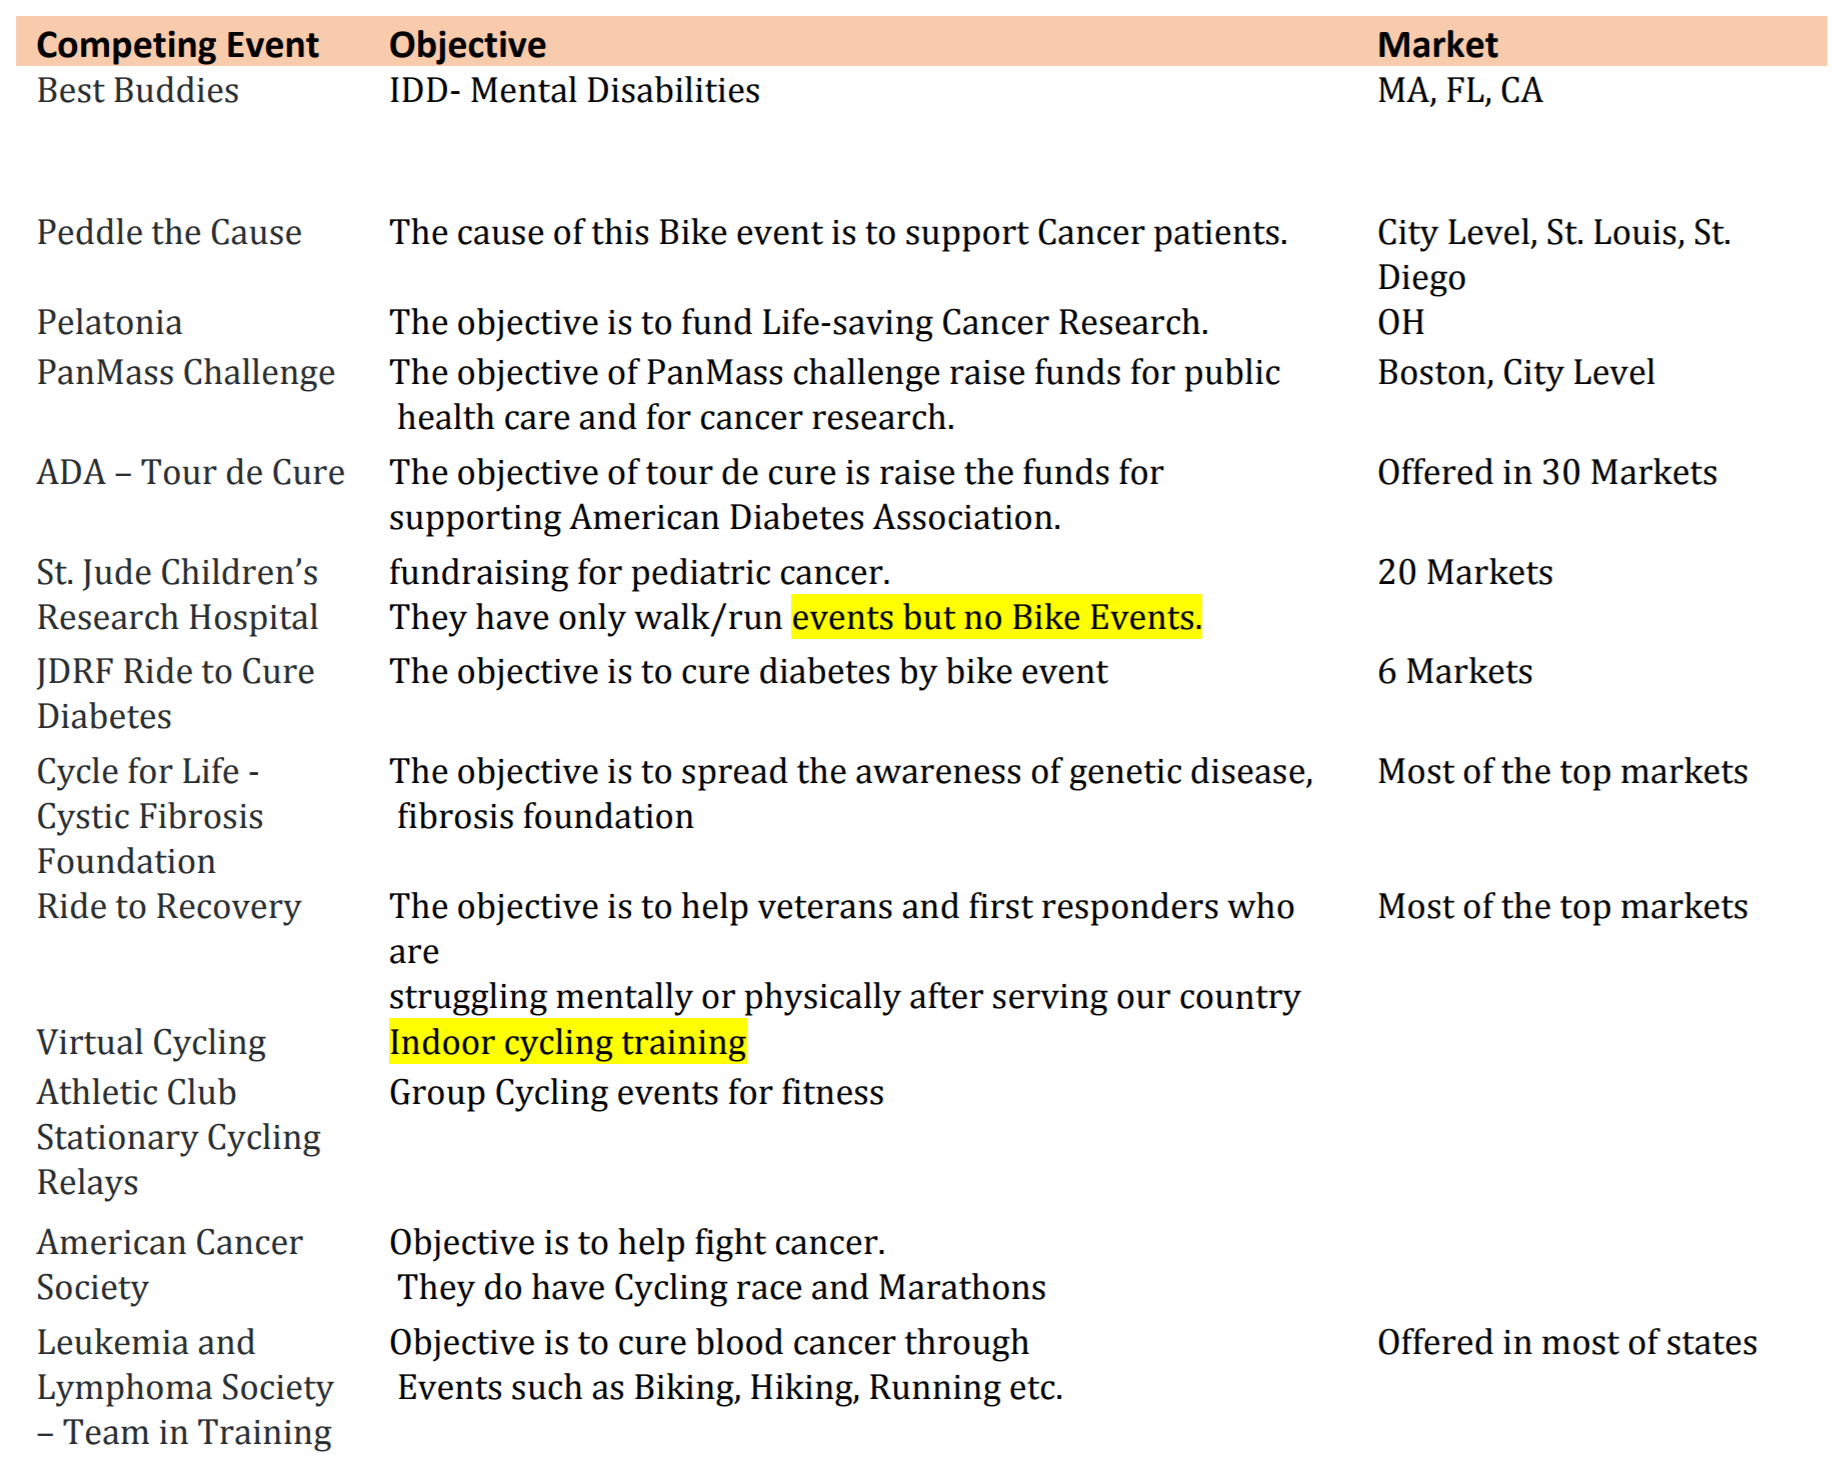
\includegraphics{competingevents.png}
\caption{Competing Events}
\end{figure}

Without any knowledge on the amount of donations and registration a
competing fundraiser is generating, we took a closer look at the
donations and participation that Bike MS generated in the states that
the competing events take place.

\begin{figure}
\centering
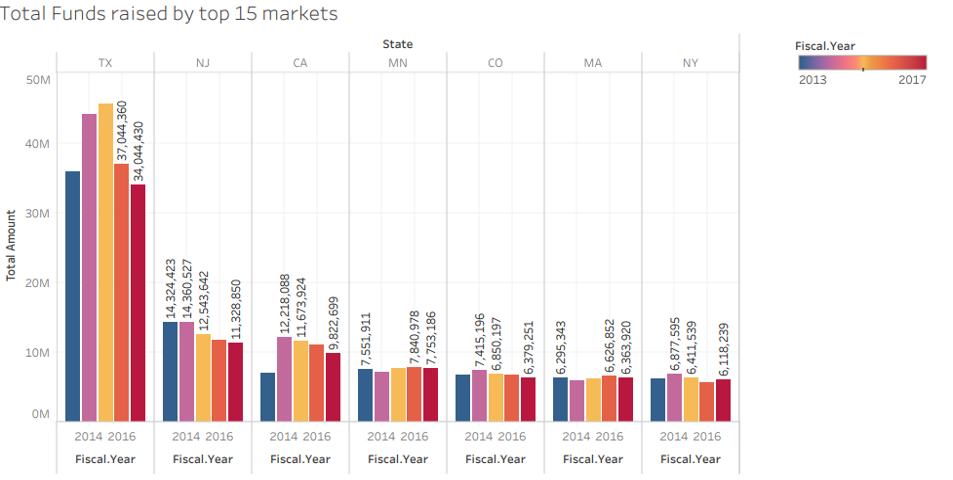
\includegraphics{fundsraisedbytopmarkets.png}
\caption{Fundraising Interaction between Competing Events}
\end{figure}

\begin{figure}
\centering
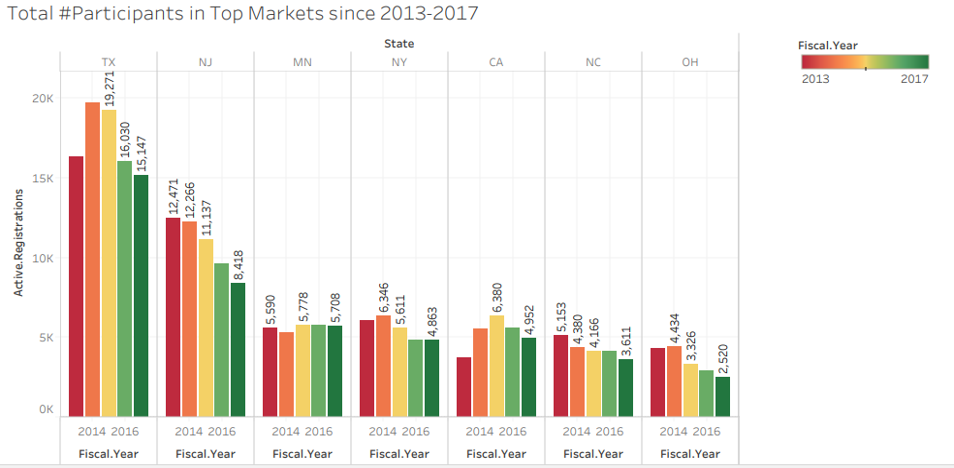
\includegraphics{participantsfromtopmarkets.png}
\caption{Participation Interaction between Competing Events}
\end{figure}

It's difficult to attribute the decrease in overall participation and
donations in a particular market to the saturation of cycling
fundraisers or competing events. Best Buddies is one of the biggest
competitors in this arena and their biggest event, the Hyannis Port
Challenge, is held in Massachusetts. The most obvious way of quantifying
the effect Best Buddies has on Bike MS events is to analyze the
surrounding

\begin{Shaded}
\begin{Highlighting}[]
\NormalTok{bestbudsHP <-}\StringTok{ }\NormalTok{bestbudsHP }\OperatorTok\StringTok{ }\NormalTok{dplyr}\OperatorTok{::}\KeywordTok{select}\NormalTok{(}\KeywordTok{everything}\NormalTok{()) }\OperatorTok\StringTok{ }
\StringTok{    }\NormalTok{dplyr}\OperatorTok{::}\KeywordTok{group_by}\NormalTok{(}\StringTok{`}\DataTypeTok{Security Category Name}\StringTok{`}\NormalTok{) }\OperatorTok\StringTok{ }\NormalTok{dplyr}\OperatorTok{::}\KeywordTok{filter}\NormalTok{(State }\OperatorTok\StringTok{ }
\StringTok{    }\NormalTok{HPradius)}

\NormalTok{bestbudsgroup <-}\StringTok{ }\NormalTok{bestbudsHP }\OperatorTok\StringTok{ }\NormalTok{dplyr}\OperatorTok{::}\KeywordTok{select}\NormalTok{(}\StringTok{`}\DataTypeTok{Fiscal Year}\StringTok{`}\NormalTok{, }
    \StringTok{`}\DataTypeTok{Security Category Name}\StringTok{`}\NormalTok{, }\StringTok{`}\DataTypeTok{Active Registrations}\StringTok{`}\NormalTok{) }\OperatorTok\StringTok{ }\NormalTok{dplyr}\OperatorTok{::}\KeywordTok{group_by}\NormalTok{(}\StringTok{`}\DataTypeTok{Security Category Name}\StringTok{`}\NormalTok{, }
    \StringTok{`}\DataTypeTok{Fiscal Year}\StringTok{`}\NormalTok{) }\OperatorTok\StringTok{ }\NormalTok{dplyr}\OperatorTok{::}\KeywordTok{summarise}\NormalTok{(}\StringTok{`}\DataTypeTok{Active Registrations}\StringTok{`}\NormalTok{ =}\StringTok{ }\KeywordTok{sum}\NormalTok{(}\StringTok{`}\DataTypeTok{Active Registrations}\StringTok{`}\NormalTok{))}

\NormalTok{bestbudsHP.viz <-}\StringTok{ }\KeywordTok{ggplot}\NormalTok{(bestbudsHP, }\KeywordTok{aes}\NormalTok{(}\DataTypeTok{x =} \StringTok{`}\DataTypeTok{Fiscal Year}\StringTok{`}\NormalTok{, }\DataTypeTok{y =} \StringTok{`}\DataTypeTok{Active Registrations}\StringTok{`}\NormalTok{)) }\OperatorTok{+}\StringTok{ }
\StringTok{    }\KeywordTok{geom_bar}\NormalTok{(}\KeywordTok{aes}\NormalTok{(}\DataTypeTok{fill =} \StringTok{`}\DataTypeTok{Security Category Name}\StringTok{`}\NormalTok{), }\DataTypeTok{stat =} \StringTok{"identity"}\NormalTok{, }
        \DataTypeTok{position =} \KeywordTok{position_dodge}\NormalTok{()) }\OperatorTok{+}\StringTok{ }\KeywordTok{geom_smooth}\NormalTok{(}\KeywordTok{aes}\NormalTok{(}\DataTypeTok{colour =} \StringTok{"lm"}\NormalTok{), }
    \DataTypeTok{method =} \StringTok{"lm"}\NormalTok{, }\DataTypeTok{se =} \OtherTok{FALSE}\NormalTok{)}
\NormalTok{bestbudsHP.viz }\OperatorTok{+}\StringTok{ }\KeywordTok{labs}\NormalTok{(}\DataTypeTok{title =} \StringTok{"Effect of Best Buddies on Northeast Market"}\NormalTok{)}
\end{Highlighting}
\end{Shaded}

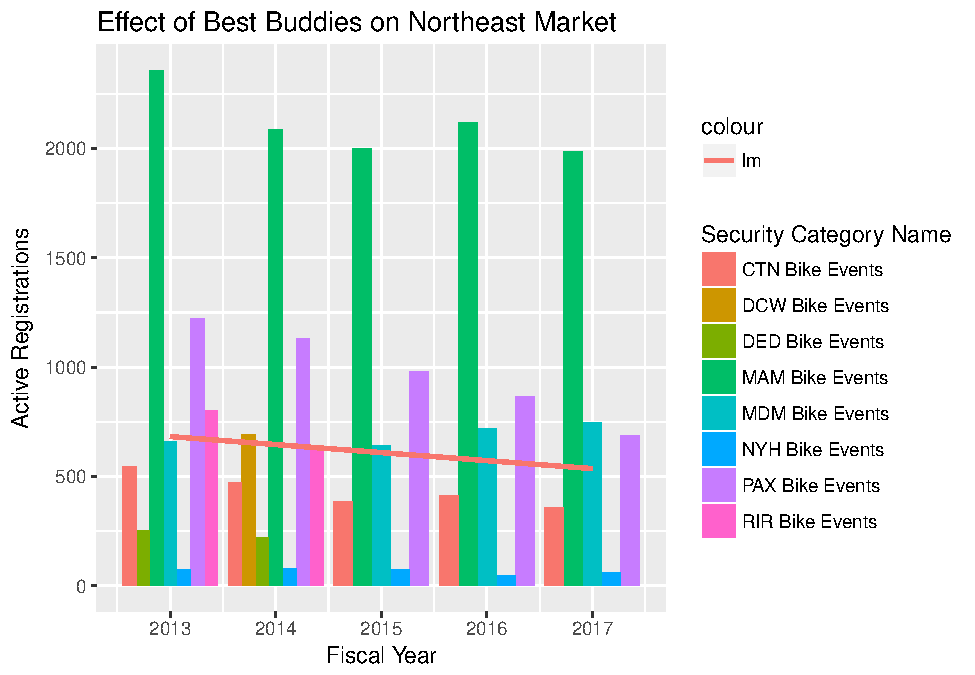
\includegraphics{index_files/figure-latex/bestbuddies-1.pdf}

\begin{Shaded}
\begin{Highlighting}[]
\NormalTok{bestbudsgroup.viz <-}\StringTok{ }\KeywordTok{ggplot}\NormalTok{(bestbudsgroup, }\KeywordTok{aes}\NormalTok{(}\DataTypeTok{x =} \StringTok{`}\DataTypeTok{Fiscal Year}\StringTok{`}\NormalTok{, }
    \DataTypeTok{y =} \StringTok{`}\DataTypeTok{Active Registrations}\StringTok{`}\NormalTok{, }\DataTypeTok{colour =} \StringTok{`}\DataTypeTok{Security Category Name}\StringTok{`}\NormalTok{)) }\OperatorTok{+}\StringTok{ }
\StringTok{    }\KeywordTok{geom_point}\NormalTok{() }\OperatorTok{+}\StringTok{ }\KeywordTok{geom_line}\NormalTok{()}
\NormalTok{bestbudsgroup.viz}
\end{Highlighting}
\end{Shaded}

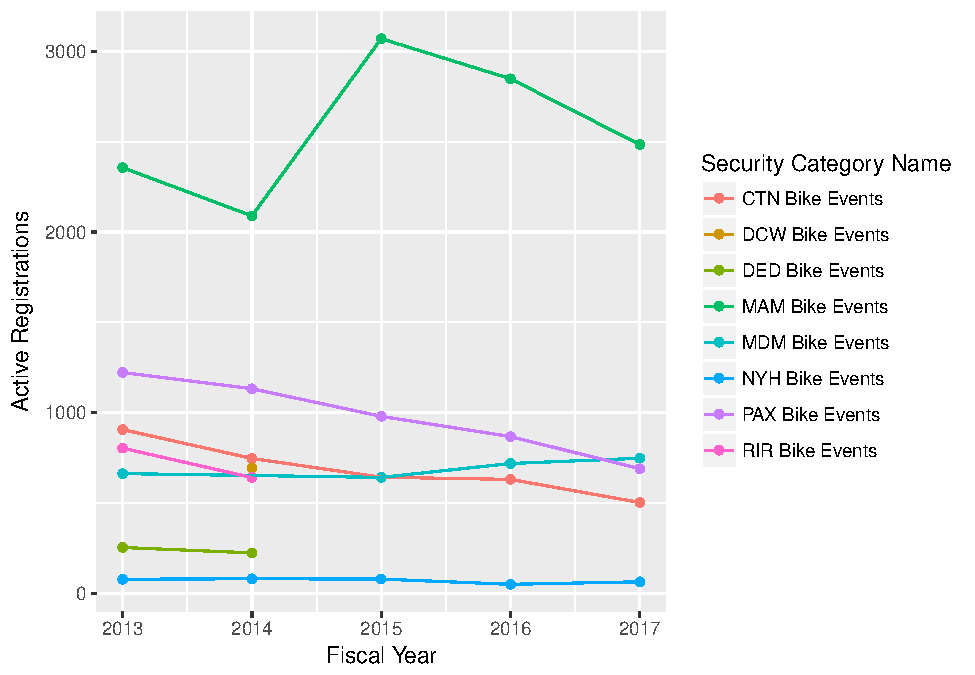
\includegraphics{index_files/figure-latex/bestbuddies-2.pdf}

These two visualizations in parallel provide the perfect insight into
how Best Buddies is effecting Bike MS metrics. We are able to see that
specifically in Massachusetts, where the Hyannis Port Challenge is held,
there is no significant change in active registrations from 2014 to
2017. We have fit a line to the average registration and see a slight
decline from 2013 to 2017, but we do not believe this to be a function
of Best Buddies' impact.

\hypertarget{what-are-the-greatest-opportunities-for-digital-marketing-investments-where-have-we-seen-the-greatest-roi}{%
\subsection{What are the greatest opportunities for digital marketing
investments? Where have we seen the greatest
ROI?}\label{what-are-the-greatest-opportunities-for-digital-marketing-investments-where-have-we-seen-the-greatest-roi}}

Bike MS uses three main channels or platforms to engage their target
market - Social, Display Ads, and Search Engine. Using their marketing
reports from 2015 to 2017 we were able to see the growth of each
platform and conversion rates that were recorded due to the budget
increase for each channel. There was a direct correlation between the
amount of money spend on social media platforms and total conversions.
Registration was the metric used to describe conversion. Here is the
breakdown of conversions per channel:

\begin{figure}
\centering
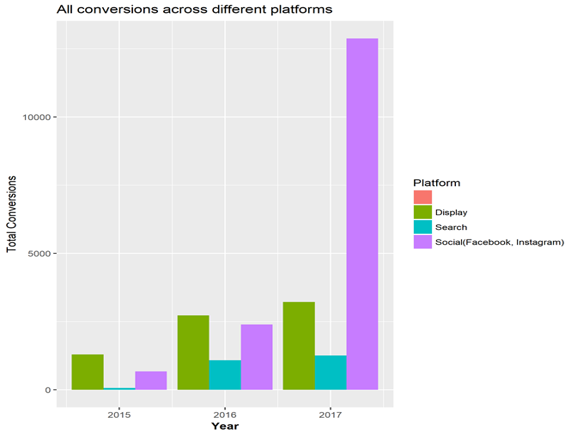
\includegraphics{digitalmarketing.png}
\caption{Digital Marketing}
\end{figure}

From 2016 to 2017 Bike MS allocated 75\% of their digital marketing
budget to social media and the remaining 25\% display ads and search
engine. Judging by the conversion from social media they saw in 2017
their return on investment was positive and we would recommend that they
continue prioritizing social media as the primary source of digital
marketing.

\hypertarget{conclusion}{%
\section{Conclusion}\label{conclusion}}

Our data-driven insights conclude that there are major growth
opportunities targeting the female population and workforce. The
prevalence of multiple sclerosis and those with personal connections to
it can have a significant impact on the future of this large fundraiser.
In the Northeastern states where Bike MS events are most successful and
MS prevalence is highest, teams from large healthcare organizations can
drive up female registration and donations. We see the gender gap in
participation as the biggest weakness. Bike MS will continue to see
positive interaction or conversion through Social Media platforms as
their main channel of digital marketing -- especially as the millennial
population begins to find job stability.


\end{document}
